\def\year{2020}\relax

\documentclass[letterpaper]{article} %DO NOT CHANGE THIS
\usepackage{aaai20}  %Required
\usepackage{times}  %Required
\usepackage{helvet}  %Required
\usepackage{courier}  %Required
\usepackage{url}  %Required
\usepackage{graphicx}  %Required
\frenchspacing  %Required
\setlength{\pdfpagewidth}{8.5in}  %Required
\setlength{\pdfpageheight}{11in}  %Required
\setcounter{secnumdepth}{0}  
\usepackage{subfigure}
\usepackage{xcolor}
\usepackage[linesnumbered,ruled]{algorithm2e}
\usepackage{amsmath}
\usepackage{dblfloatfix}    % To enable figures at the bottom of page
\usepackage{setspace}
\usepackage{tikz}
\usetikzlibrary{positioning}

\makeatletter
\newcommand{\removelatexerror}{\let\@latex@error\@gobble}
\makeatother
\begin{document}
% The file aaai.sty is the style file for AAAI Press 
% proceedings, working notes, and technical reports.
%
\title{A Genetic Approach to the Formulation of Tetris Engine}
\author{Jiachen Zhang, Miaoqi Zhang, Shuheng Cao\\
\{j756zhan, m337zhan, s53cao\}@uwaterloo.ca\\
University of Waterloo\\
Waterloo, ON, Canada\\
}
\maketitle
\newcommand\bi[1]{{\textcolor{black}{#1}}}
\newcommand\blue[1]{\textcolor{blue}{\textbf{#1}}}
%%%%%%%%%. Abstract %%%%%%%%%

% \begin{abstract}
% % {\bf Complete this section for D4.}

% % The {\it Abstract} should be at most 150 words long, and should summarize briefly what your project is about.  This includes the motivation for the problem (2-3 sentences), the problem you tackled (2-3 sentences), and your main results (1-2 sentences).   
% \end{abstract}

%%%%%%%%%. Introduction %%%%%%%%%
\section{Introduction} 

% The {\it Introduction} section ($\sim$1 page) describes the background and motivation behind your work, and provides an overview of the work and the findings.  It should include the following content.  
%
\begin{itemize} 

  \item 
  {\bf Motivations}
  % {\bf Complete this part for D1.}
  
  % Motivate your entire paper.  At a high level, describe the problem that your project is addressing.  Why is this an important problem to tackle?  If there a solution to this problem, what are some potential real-world impacts of this solution?  Try to give a compelling motivating story.  If possible, support your argument with evidence such as facts and statistics.  (2-3 paragraphs)
  
  With the great triumph of AlphaGo in 2016, more and more researchers are interested in using machine learning techniques to solve more advanced and complicated games such as StarCraft II. However, in the authors' opinion, it also provides us \bi{with} an invaluable opportunity to revisit some of the traditional video games, \bi{where we aim} for more reliable and satisfying results. Consequently, \blue{this project's primary motivation is to introduce, implement, and compare several different approaches to tackle the Tetris}, a tile-matching video game with enduring appeal and popularity. \bi{In brief, Tetris is a tile-matching video game where the player will rotate and place seven different kinds of Tetrominos on top of each other. Horizontal lines will be cleaned up once they are complete, and a score will be awarded for that. This game's ultimate goal is to achieve as many marks as possible before the pieces reach the top of the game board, and therefore, there is no victory in this game.}
  
  Solving Tetris is a crucial and intriguing topic due to the two reasons below. On the one hand, Tetris is essentially an extraordinary optimization problem because each game will end no matter how well \bi{the Tetrominos} are placed \cite{burgiel_1997}. \bi{As a result}, there is no such thing as perfect solutions to Tetris and there is always room to improve. On the other hand, the analyses and comparisons mentioned in this report are not limited to Tetris only, where we could broaden them to real-life problems, such as self-driving cars and robotics, \bi{with appropriate modifications on the architectures introduced in this article}.
  
  Finally, \bi{solving a relatively simple game like Tetris will help us better understand the related Reinforcement Learning models.} One of the main problems the machine learning community faces is the lack of explainability and interpretability for most of the models. The direct analyses on most of the recent models, such as AlphaGo and AlphaZero, are notoriously complicated and challenging, but with a more straightforward and simplified setup like Tetris, it gives us more opportunities to have a more in-depth insight into what is happening under the hood. Consequently, the results from simple setups will contribute to a better and deeper understanding of the more complex models.
  
  \item 
  {\bf Methodologies}
  % {\bf For D1, describe the problem and your methodologies only.  Then, complete this part for D4. }
  
  \bi{The problem we are trying to solve is to design an agent that could achieve as many scores as possible in the Tetris game. We will implement three algorithms, including the baseline method, as shown below.}
  % Describe, at a high-level, the problem you tackled and your main results.  What research questions are you trying to answer?   What methodologies did you used to answer the question? What are the performance measures that you used to evaluate the methodologies?   Describe your key findings in 2-3 sentences. (2-3 paragraphs)
  % In brief, the methodology of this project consists of four main parts, as shown below.
  \begin{itemize}
    \item 
    First and foremost, we built a Tetris interface for both visualization and training purposes. For the sake of communication with our models, the interface is written in Python \bi{and it will support two basic functionalities: 
    \begin{itemize}
      \item Generating all the successors for current state.
      \item Calculating score or reward for each state.
    \end{itemize}}
    \item 
    Next, we \bi{will solve} the problem using a hand-crafted agent. \bi{Inspired by Bertsekas and Tsitsiklis's paper} \cite{Bertsekas_1996}, we will manually chose the weights for 4 most representative state features: the number of holes, the height of the highest column, the height of each column, and the difference in height between consecutive columns. This approach is based mainly on the heuristic search algorithm and involves a lot of trails-and-errors. The result serves as the benchmark for the project \bi{using the evaluation metrics mentioned below}.
    \item 
    On top of that, we will also tackle the problem \bi{using local search algorithm}. The main idea is to use a genetic algorithm to automatically find an optimal weight combination for 9 state features, where the detailed description for the features could be found in the Methodology section. 
    % \bi{According to the nature of the local search algorithm, this method will find the optimal weights without any human interference, and consequently, it is able to rely on more state features compared with the hand-crafted agent. As a result, we expect the local search algorithm to outperform the benchmark.}
    
    % After 200 training epochs, we indeed get a result surpassed the benchmark.
    \item \bi{Ultimately, we will solve the problem with reinforcement learning. The main idea is that we will build and train a deep Q-network (DQN) to evaluate all the successor states of the current state. More precisely, the DQN will receive a bitmap representation of successor and output a non-negative number represents the score for it. After that, the agent will choose the successor with the highest score with probability $\epsilon$ and otherwise, it will select a random successor.}
    % Ultimately, we added more functionalities to the traditional Tetris, like introduce the ability to see the next Tetromino and enable holding the unwanted Tetromino, and the retrained model yields satisfying results, which proved the ability to generalization.
  
\end{itemize}
{As for the evaluation metric, we will use the number of lines cleaned up before game over as our primary metric so that we could compare the three methods with each other as well as implementations from other papers. One thing worth mention is that in the DQN training, we won't directly use the evaluation metric mentioned above as the reward because it is too sparse. Instead, we will design a reward that is positively correlated with the evaluation metrics. More concretely, we will use the following rewarding scheme:}
\begin{itemize}
  \item Game over gives $-100$.
  \item Cleaning up $k$ lines gives $10k^{2}$.
  \item Safely landing a piece gives $1$.
\end{itemize}
% \begin{table}[h!]
%   \centering
%   \normalsize{
%     \begin{tabular}{ |c|c| } 
%       \hline
%       Situation & Reward  \\ 
%       \hline
%        Game over & $-100$  \\ 
%        \hline
%        Clean up $k$ lines & $10\times k^{2}$  \\ 
%        \hline
%        Safely landing a piece & $1$  \\
%       %  \hline
%       %  Otherwise & $0$  \\
%        \hline
%       \end{tabular}}
%   \caption{Reward Function}
%   \label{tab:reward}
% \end{table} 

% \item 
% {\bf Complete this bullet point for D4.}

% Emphasize your contributions.  How should we interpret the results?  Why should people care about this work?   Does this project introduce any novel techniques or reveal any unexpected findings?  In bullet point forms, list 3-4 key contributions of your project.

\end{itemize}

%%%%%%%%%. Related Work %%%%%%%%%

\section{Related Work} 

There is a number of algorithms about Tetris so far. Most algorithms for Tetris use features and a linear evaluation function \cite{SO19}. The algorithms define multiple features and assign a weight value to each of the features. For a specific state with an existing Tetromino, it will use the evaluation function to calculate the evaluation value according to the weight of the features for every possible states. And then a "best" placement of the Tetromino will be picked according to the evaluation value.

Tracing back to 1996, J.N. Tsitsiklis and B. Van Roy formulated Tetris as a Markov Decision problem. They introduced Feature-Based Method for Large Scale Dynamic Programming. The algorithm introduced two features, which were the number of "holes" and the height of the tallest column. Each state will be represented as a two-hundred-dimensional binary vector since the Tetris board is form by $10 \times 20$ grids. And a seven-dimentional bianry vector will represent the current falling Tetromino since there are seven type of Tetrominos in total. The algorithm can eliminate 31 rows on average of a hundred games \cite{TV96}.

Later on, more features have been taken into consideration. For example, peak height, landing height, number of holes, row transition, column transition and eroded piece cells \cite{WCWT}. 

These features were identified by the best artificial Tetris player until 2008 and introduced evalutation function: 
$-4 \times holes - cumulative\ cells - row\ transitions - column\ transitions - landing\ height + eroeded\ cells$ \cite{SO19}. However, most algorithm will perform a row elimination whenever it is possible. This is not optimal in the long term because there could be some state that multiple rows can be eliminated at once \cite{WCWT}. 

Tsai, Yen, Ma and Yu implemented "Tetris A.I.". Scores will be rewarded if a I-Tetromino is dropped and 4 rows are eliminated. The main idea is to make this kind of move as many as possible. The solution for this is to stack on the 9 columns and remain the left column empty. As long as an I-Tetromino apprears, it will be drop at that seperate column to eliminate multiple rows \cite{WCWT}.

Moreover, they also implemented another model called "Two Wide Combo A.I.", which is a little bit more complex than the previous algorithms. It breaks the process into two parts. One is to "Stack" on the left eight columns by using BFS, and the other part is "Combo", which is to eliminate rows consecutively to earn Combo Bonus by dropping Tetrominos into the rest two columns \cite{WCWT}.

The use of generic algorithm provides a new way which is worth taking into consideration. In 2006, Szita and Lorincz implemented cross-entropy algorithm. New features were introduced and for each feature, multiple games were played. It took the mean and standard deviation of the best weight of the linear policy that maximize the score and generated a new generation of policies \cite{SO19}.

Back in 2003, Thomas Gärtner, Kurt Driessens and Jan Ramon introduced a new approach to Tetris optimization\cite{s017}. What's innovative in this paper is that researchers primarily used Relational Reinforcement Learning (RRL), training the network with Gaussian processes and graph kernels. Relational Reinforcement Learning advances traditional Reinforcement Learning by integrating with a relational learning programming which is also known as inductive logic programming. The use of Gaussian processes is to make probabilistic predictions and allow the agent to incrementally perform learning tasks. On the other hand, graph kernels help represent various states and actions during training process in a more structural way, which greatly facilitates learning. Compared to some previous RRL models which train data based on techniques such as decision trees, this approach has proven to be more effective.

In 2016, researcher at Stanford University continued to optimize Tetris engine performance using Reinforcement Learning \cite{s016}. They used a notation called Q function. This function evaluate actions taken by the AI at various stages/states during the game; the value of this Q function tells us what the best next action is. Researchers attempted to improve convergence of Q function with the aid of heuristic functions. This method yields the best performance when combined with grouping actions. Basically, grouping actions means the entire sequence of actions a single piece take as it drops to the bottom whereas a single action is just one movement of the piece such as one space to the left. Although grouped actions increase game length compared to single actions, they achieved a much high game score. Another technique that significantly boosts the performance is transfer learning. Transfer learning effectively scores an average of two lines per game, compared to no lines for learning from scratch. The final technique used is called prioritized sweeping. Prioritized sweeping involves calculating a priority value. Based on that value, the researchers sampled actions based on probabilities proportionally to their priorities. This technique solves several problems, for example, the issue that certain actions gotten drastically under-represented in the experience dataset.

%%%%%%%%%. Methodology %%%%%%%%%

\section{Methodology}

\subsection{Handcrafted Agent}
Our first approach is a manually trial-and-error approach, or more precisely, we will assign a weight manually for each feature below according to our intuition and experiment results. Then, for each generated successor states, we will always choose the state with the lowest heuristic value, which is calculated based on a summation of the four weighted features. Here are the four features we are going to use and a rationale for choosing them:
\begin{enumerate}
 \item {\bf number of lines cleared}\footnote{Note that this is special compared with other features because we want it to be as large as possible, so we will assign a negative weight to it.}

This feature faithfully reflects our evaluation metric since we will achieve scores only by cleaning lines.

 \item {\bf number of holes}

The holes in the Tetris game are particularly harmful because, in order to clean the line containing a hole, we need to clean up all the lines above that hole. 

 \item {\bf sum of difference of height between adjacent columns}

The "gaps" in the board make it harder to clear rows simply because the Tetrimonos are generated randomly, and those "gaps" are not likely to be filled perfectly by the next Tetrimono.

 \item {\bf maximum height}

The higher the board is, the closer it is to the "ceiling" (vertical limit of the board), which means there may be fewer steps to play before the game terminates.

\end{enumerate}

We would run simulations consecutively and record the performance associated with the weight combination. Based on the results, we would adjust one or more weight values and use them in the next simulation until the game behaves rationally in human criterion.

An advantage of this handcrafted approach is that we are somewhat informed of what features should be rewarded and penalized. Compared to adjust the weight using algorithms, manually adjustment will give us a better understanding and intuition about the game during the weight adjustment process.
\subsection{Local Search Agent}
Essentially, in a handcrafted agent approach, human decisions are used to adjust weight combinations during every iteration of the simulation. Such an algorithm obviously has some limitations because a lot of possible adjustments to the weights can not be tested/explored. Moreover, we only use four features in the handcrafted agent, which may not be sufficiently representative. As a result, we need an approach that takes more underlying features into consideration, together with a more systematical way to improve weight combinations other than just by intuition. With these goals bearing in mind, we propose a second approach that utilized the genetic algorithm, a powerful local search algorithm.

In the genetic algorithm approach, we would use a feature set that includes a total of 10 features. These features are:
\begin{enumerate}
 \item[1-4.] features same as Handcrafted agent
 \item[5.] number of blocks currently on the board
 \item[6.] number of rows with at least a hole in it
 \item[7.] max height difference between the lowest column and highest column
 \item[8.] number of cells that is not filled with no blocks above it and two horizontal neighbors filled
 \item[9.] the height where the highest hole is located
 \item[10.] number of occupied rows which is above the highest hole such that if removed, the highest hole is no longer a hole
\end{enumerate}

Now that once we have our feature set, we would construct our genetic algorithm approach start by defining the following terms:

\begin{itemize}
 \item {\bf Chromosome}: An array of 10 numbers representing our weights combination, each weight ranges from $-1$ to $1$.
 \item {\bf Fitness}: Number of lines cleared before the game ends.
 \item {\bf Selection}: After ranking each state based on fitness score, we will remove $p$ percent of states with low fitness scores and use remaining states as parents for next generation.
 \item {\bf Crossover}: Take a combination of weights among the remaining parents and make it the chromosome for the children (detailed implementation is shown below).
 \item {\bf Mutation}: After crossover, one random weight value in the chromosome of the child state will be mutated with a certain probability $q$.
\end{itemize}


The game would start by generating random chromosomes for $M$ children, and for each of these children, we will run $N$ simulations on it. The average lines cleaned will be recorded for each child and will be used as the fitness score for them. Next, we would begin our selection process, which would remove $p\%$ children and promote the remaining children to be parents. For this group of parents, we would randomly choose $M$ pairs of parents and perform crossover and mutation operations to get $M$ children for the next generation. Then, for each child in this generation, we would start the above the process all over again. That is, we would run simulation, record fitness, remove least fit offspring, and generate successors. We would stop the game until there is no significant improvement in performance between the parents and the children. Finally, we will choose the child with the highest fitness score and use its chromosome as our final weight combination. 

One important thing worth noting is the implementation of crossover. When determining the exact combination of chromosome from the parent states, we will consider the fitness scores of parents because if one parent has a higher fitness score than the other, the former chromosome should have been more optimal than the latter one. Therefore, we would want the child to "inherit" more from the first parent. Let's assume the first parent's fitness score is $f1$ and that of second parent is $f2$. Without loss of generality, assume $f1 \geq f2$, then we define the combination as follows: 
 
 \begin{itemize}
 \item if $\frac{f1}{f2} = 1$, we will randomly take 5 weights from the first parent and fill the remaining weights from the second parent.
 \item if $0 < \frac{f1}{f2} - 1 \leq 0.25$, we will do a 6:4 sampling.
 \item if $0.25 < \frac{f1}{f2} - 1 \leq  0.5$, we will do a 7:3 sampling.
 \item if $0.5 < \frac{f1}{f2} - 1 \leq  0.75$, we will do a 8:2 sampling.
 \item if $0.75 < \frac{f1}{f2} - 1$, we will do a 9:1 sampling.
 \end{itemize}


 Notice that this scheme involves many hyperparameters, such as the lower and upper bounds of the ratio, and in theory, we should determine this during our training. However, doing so will introduce too many degrees of freedom during training, and to avoid this, we will insist on this scheme.

In conclusion, in the genetic algorithm approach, we eliminate a lot of human assumptions. That is, what weight value should be changed, and by how much. We would also take into consideration more features that may further eliminate human assumptions of which feature could have an underlying impact on the game-play or not. Despite the amount of computation with this approach, we are more likely to find an optimal weight combination compared to a handcrafted agent.


\subsection{Reinforcement Learning Agent}

The genetic algorithm mentioned above is intelligent in the sense that it will automatically find optimal weight combinations. However, notice that it is still not perfect because the state features are always chosen by humans, and they are not necessarily representative. More concretely, we may lose some information since we will represent all the successors' states, which is of size $20\times 10$, using only ten features. Thus, we will develop a new algorithm that eliminates human-chosen features and finds a feasible representation itself.

As a result, we naturally lean towards the fields of reinforcement learning and will start with the Q-learning introduced by Chris Watkins in 1989. The detailed deduction and convergence proof are pretty complicated and are out of the scope of this report. However, the final results of Q-learning are incredibly similar to dynamic programming, where we maintain a Q-table with current states $s_i$ as column and available actions $a_j$ as rows (Table \ref{tab:qtable}).

$\,$
\begin{table}[h!]
  \centering
  \normalsize{
    \begin{tabular}{ |c|c|c|c|c|c| } 
      \hline
       & $a_{0}$ & $a_{1}$ & $\cdots$ & $a_{n}$  \\ 
      \hline
       $s_{0}$ & $0.91$ & $0.65$ &$\cdots $ &$0.45$  \\ 
       \hline
       $s_{1}$ & $0.86$ & $0.14$ &$\cdots $ &$0.19$  \\ 
       \hline
       $\vdots$ & $\vdots$ & $\vdots$ &$\ddots $ &$\vdots$  \\ 
       \hline
       $s_{m}$ & $0.26$ & $0.61$ &$\cdots $ &$0.27$  \\ 
       \hline
      \end{tabular}}
  \caption{Q-table example with random initialization}
  \label{tab:qtable}
\end{table}

And for each step, we will update the entry $(s_{t}, a_{t})$ using the formula

\[
    % Q^{new}(s_{t},a_{t}) \leftarrow \underbrace{Q(s_{t},a_{t})}_{\textit{old value}} + \underbrace{\alpha}_{\textit{learning rate}} \cdot  \overbrace{\bigg( \underbrace{\underbrace{r_{t}}_{\textit{reward}} + \underbrace{\gamma}_{\textit{discount factor}} \cdot \underbrace{\max_{a}Q(s_{t+1}, a)}_{\textit{estimate of optimal future value}}}_{\textit{new value (temporal difference target)}} - \underbrace{Q(s_{t},a_{t})}_{\textit{old value}} \bigg) }^{\textit{temporal difference}}
    Q(s_{t},a_{t}) \leftarrow (1-\alpha) Q(s_{t},a_{t}) + \alpha   \left ( r_{t} + \gamma  \max_{a}Q(s_{t+1}, a)\right ) 
\]
where we have two hyper-parameters embedded in this formula:
\begin{itemize}
  \item $\alpha$: learning rate, which determines to what extent newly acquired information overrides old information.
  \item $\gamma$: discount factor, which determines the importance of future rewards.\footnote{The term $\max_{a}Q(s_{t+1}, a) $ represents the estimation of the optimal future value.}
\end{itemize}

On top of that, we also need to manually determine three important setups:
\begin{itemize}
  \item $s_{i}$: all the possible states for the environment represented by a $20\times 10$ bitmap.
  \item $a_{j}$: all the possible actions a player can take for a state.
  \item $r_{t}$: reward received when moving from the state $s_{t}$ to $s_{t+1}$ and is determined by the reward function.
\end{itemize}

With all these hyper-parameters and setups, we will let the agent interact with the environment on its own. At each state, the agent will always choose to perform the action with the highest Q-value and update the Q-table according to the updating formula.\footnote{Here, it is not always true that the agent will perform the action with the highest Q-value. Some techniques like $\epsilon$-greedy will choose the optimal action with probability $\epsilon$ and a random walk otherwise. We will talk more about this later in this section.} We will stop Q-learning until the agent completes the game, and repeat this process for large enough epochs so that the Q-table converges.



Now, we will begin with a naive adaptation to the Tetris by defining states to be all the possible game states for a Tetris board of size $20\times 10$ and defining actions to be the set $\{clockwise\,\,rotation$, $counter\textit{-}clockwise\,\,rotation$, $left$, $right$, $down\}$.
% $\{\textit{left},\textit{right}, \textit{down},\textit{clockwise rotation}, \textit{counter-clockwise rotation}\}$.

Theoretically, we could tackle this Tetris problem directly using the Q-learning setups mentioned above, but we are facing two severe hindrances:
\begin{enumerate}
  \item The reward is very sparse because all the actions except {\it down} are perfectly reversible. For example, $left$ can be reversed by $right$, and $clockwise\,\,rotation$ can be reversed by $counter\textit{-}clockwise\,\,rotation$. As a result, in the exploration stage, it will take the agent a long time before it can achieve a reward\footnote{Notice that according to the Table \ref{tab:reward}, we will only get a reward when we place a Tetromino so we won't get anything during the placement process.}, which is particularly bad for training purposes.
  \item Furthermore, according to Phon-Amnuaisuk's paper, the number of stable states for a $20\times 10$ Tetris board is in the order of $10^{60}$ \cite{somnuk_2015}, which means our Q-table will be of size approximately $5\times 10^{60}$. This table is way too large to store in RAM and the training time for such a large table is also unbearable.
\end{enumerate}

Now, we will conquer these two hindrances and develop a practical architecture for this problem. For the first one, inspired by Stevens's idea of \textit{grouped action} \cite{Stevens_2016}, we can leverage the successor function from the genetic algorithm and reduce the dimension of Q-table. More precisely, instead of defining action $a_i$ to be one of the $5$ single moves, we will use a \textit{grouped action} to represents a sequence of moves until the current Tetromino is landing.\footnote{In other words, each \textit{grouped action} refers to a final placement for a specific Tetromino.} For example, if we got an L-shape Tetromino as shown in Figure \ref{fig:grouped_action}, one potential \textit{grouped action} will be $\{left\times 3, \,\,clockwise\,\,rotation \times 1,\,\,down\times 10\}$, which is essentially the successor function used in the genetic algorithm.

% \begin{figure}[h!]
%   \centering
%   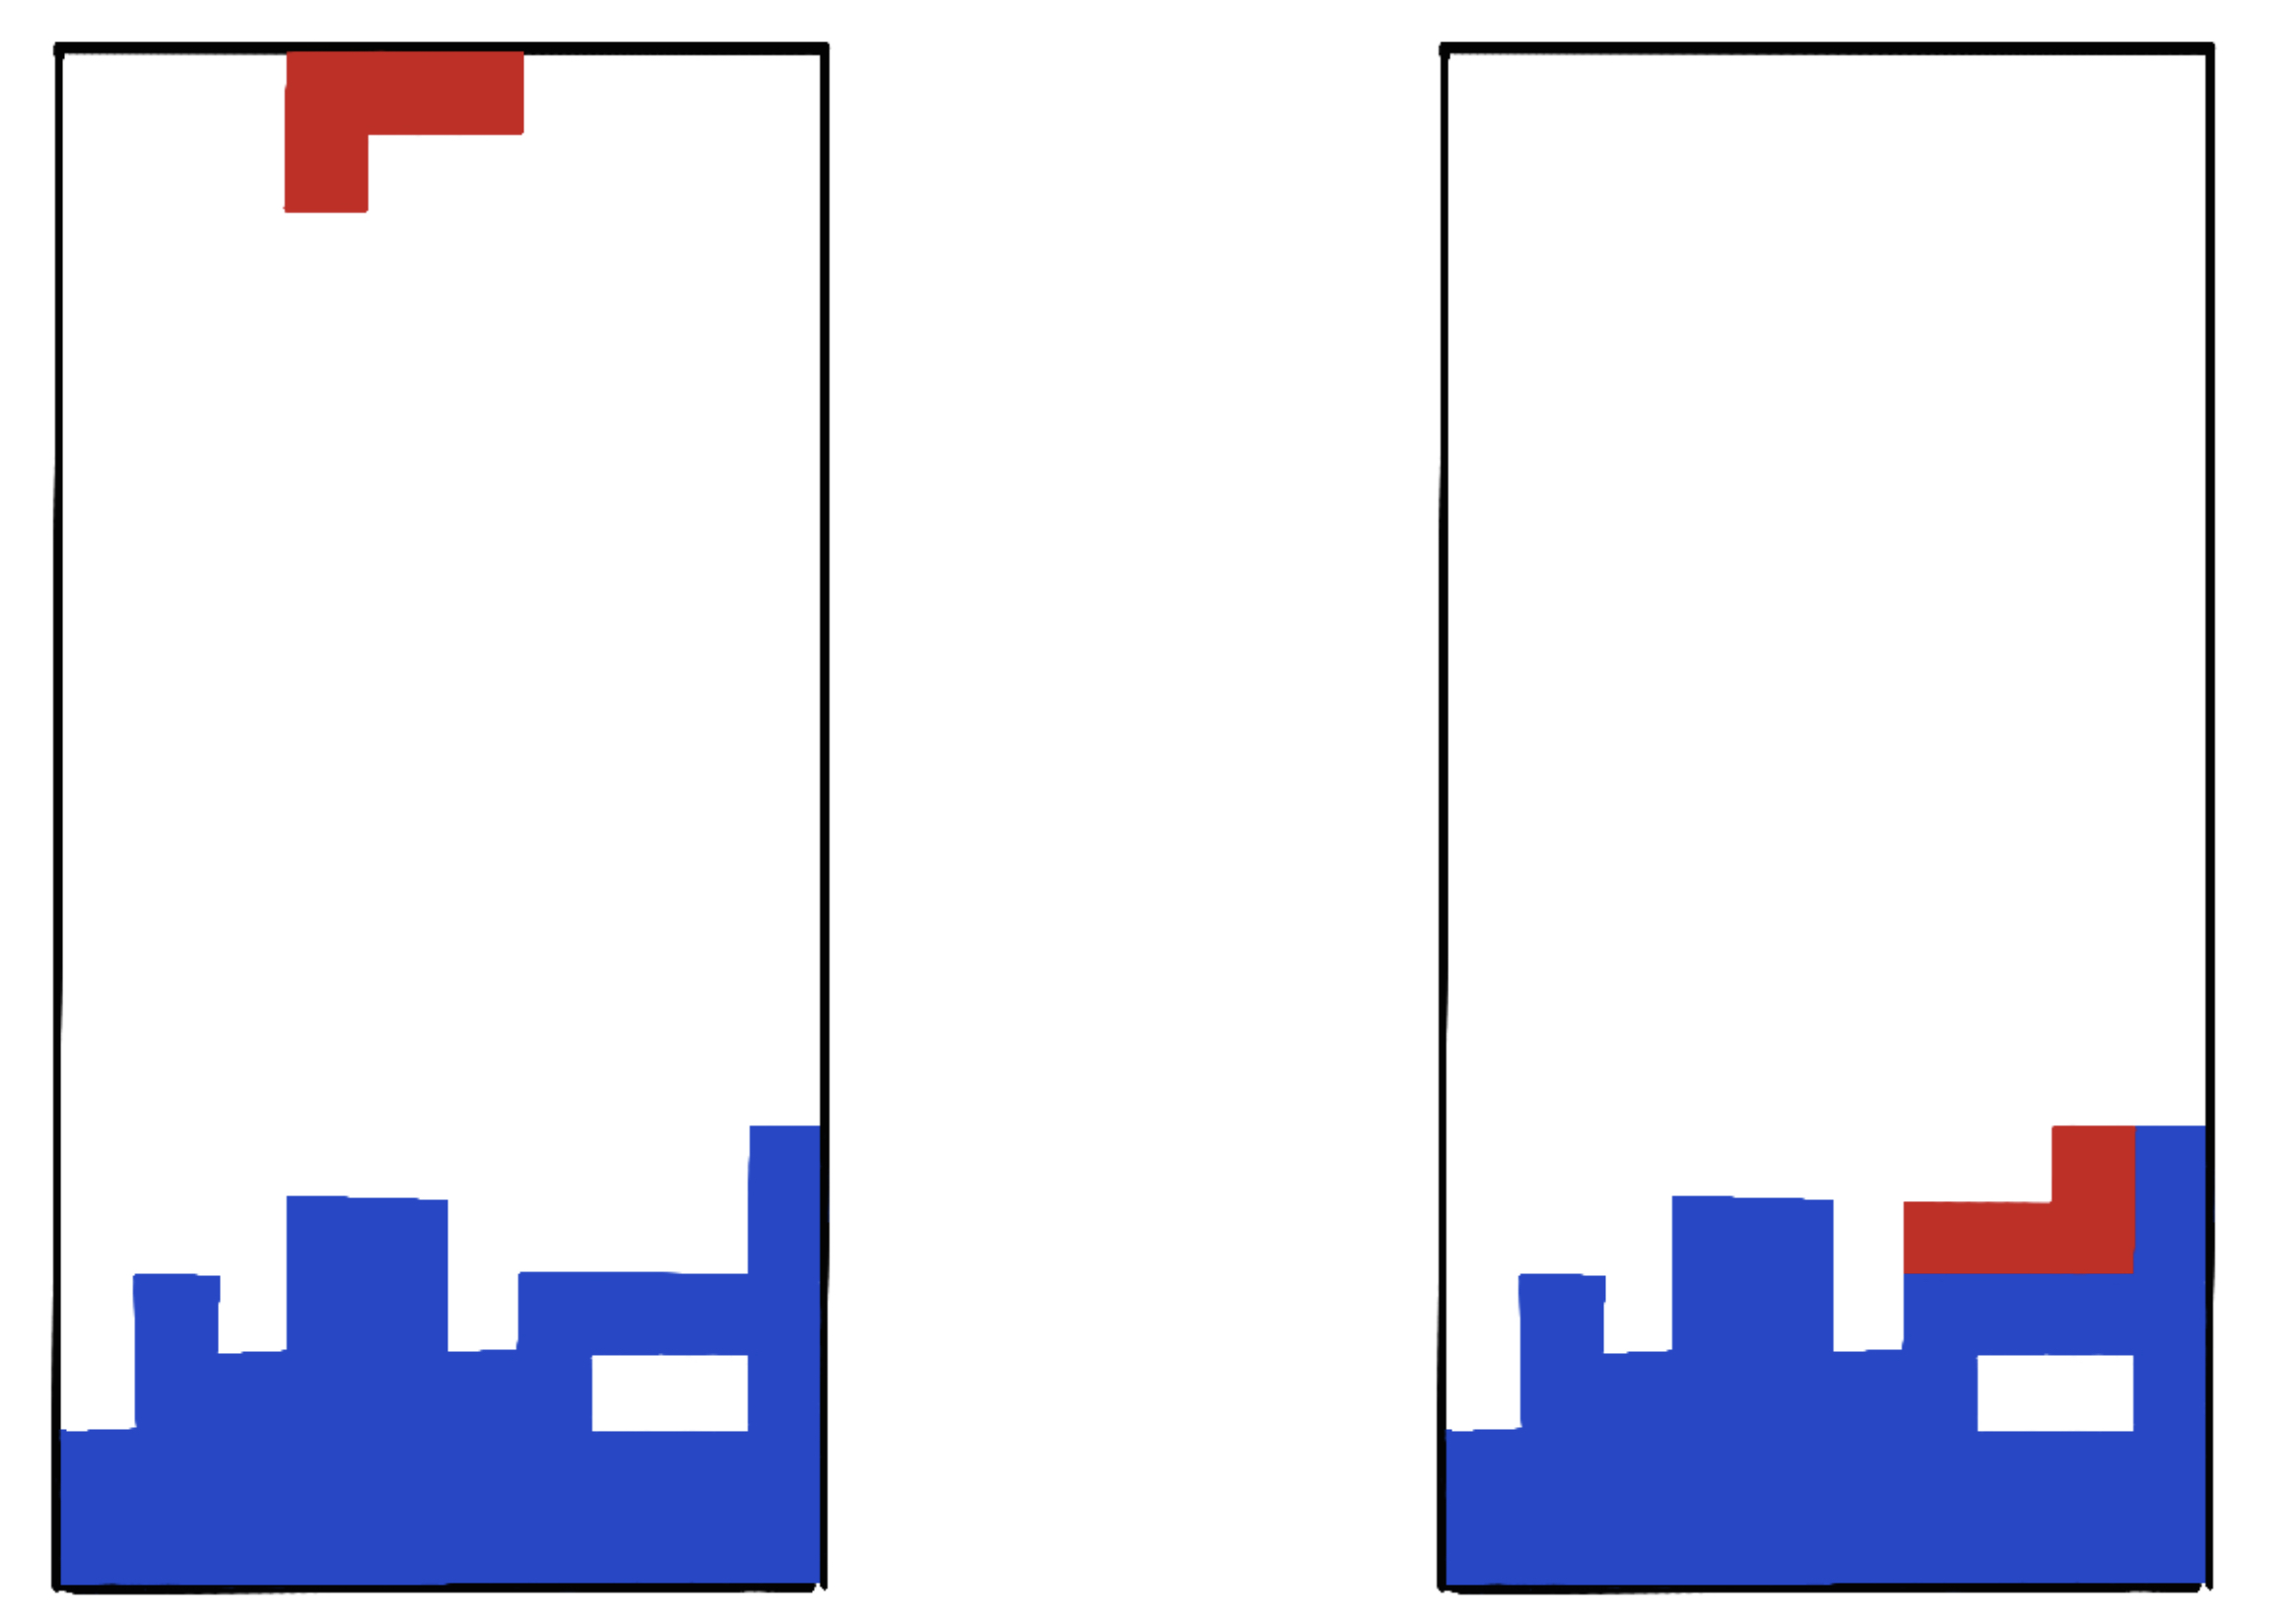
\includegraphics[width=0.9\linewidth]{figures/group_actions.jpeg}
%   \caption{Grouped action example}
%   \label{fig:grouped_action}
% \end{figure}
\begin{figure}[t!]
  \centering
  \subfigure{
  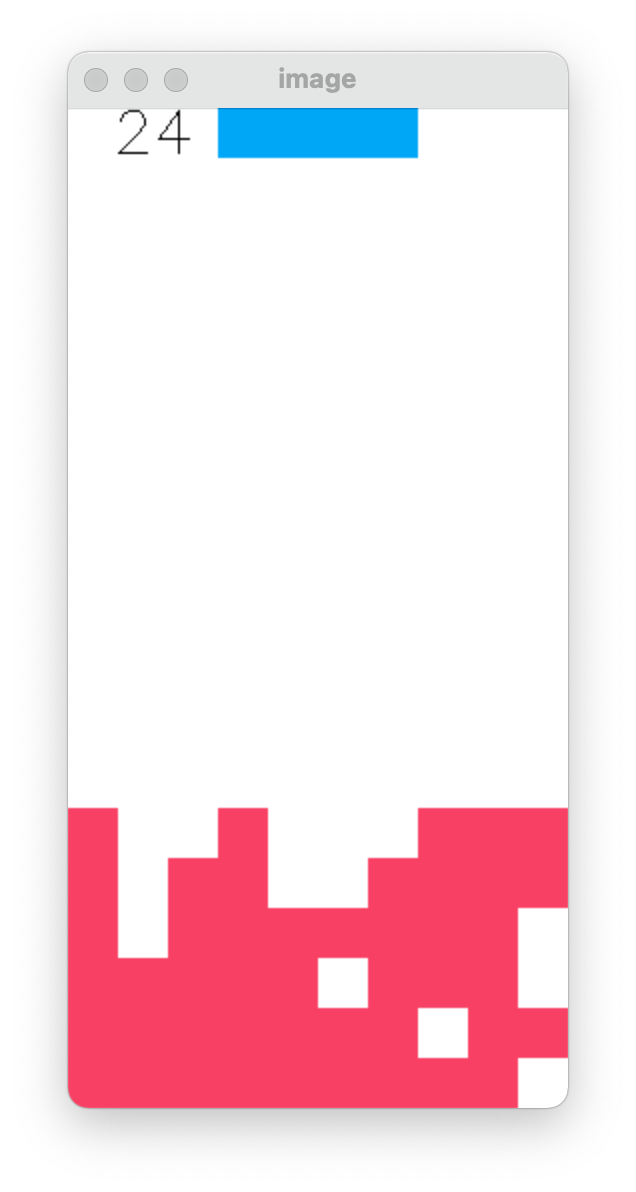
\includegraphics[width=0.22\textwidth]{figures/group_action1.png}
  }\hfill
  \subfigure{
  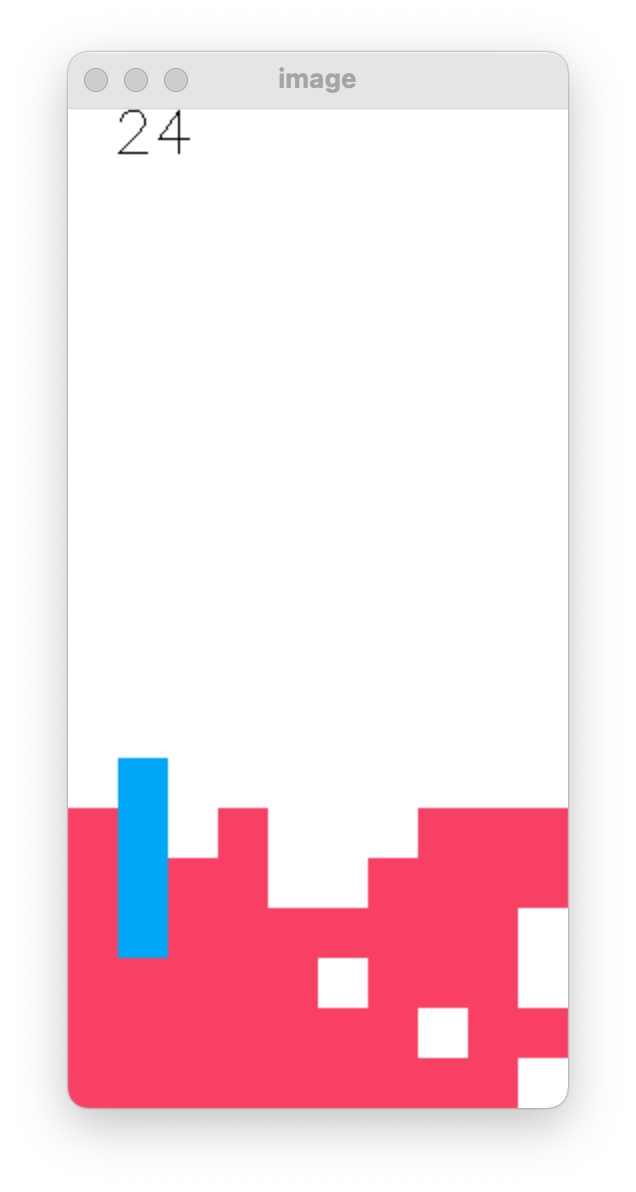
\includegraphics[width=0.22\textwidth]{figures/group_action2.png}
  }
  \caption{Grouped action example}
  \label{fig:grouped_action}
\end{figure}

With the new definition of \textit{grouped action}, we can reconstruct our Q-table and rewrite our updating formula. Notice that because after each grouped action, it's guaranteed to be a stable state (i.e., there is no floating Tetromino), we can simplify the two-dimensional Q-table (Table \ref{tab:qtable}) into one-dimensional (Table \ref{tab:newqtable}).

\begin{table}[h!]
  \centering
  \normalsize{
    \begin{tabular}{ |c|c|c|c|c|c| } 
      \hline
      $s_{0}$ & $s_{1}$ & $\cdots$ & $s_{m-1}$ & $s_{m}$  \\ 
      \hline
      $0.91$ & $0.65$ &$\cdots $ &$0.45$ &$0.19$  \\ 
       \hline
      \end{tabular}}
  \caption{New Q-table with random initialization}
  \label{tab:newqtable}
\end{table}

with the modified updating formula:
\[
    % Q^{new}(s_{t},a_{t}) \leftarrow \underbrace{Q(s_{t},a_{t})}_{\textit{old value}} + \underbrace{\alpha}_{\textit{learning rate}} \cdot  \overbrace{\bigg( \underbrace{\underbrace{r_{t}}_{\textit{reward}} + \underbrace{\gamma}_{\textit{discount factor}} \cdot \underbrace{\max_{a}Q(s_{t+1}, a)}_{\textit{estimate of optimal future value}}}_{\textit{new value (temporal difference target)}} - \underbrace{Q(s_{t},a_{t})}_{\textit{old value}} \bigg) }^{\textit{temporal difference}}
    Q(s_{t}) \leftarrow (1-\alpha) Q(s_{t}) + \alpha   \left ( r_{t} + \gamma  \max_{s_{i} \in successor(s_{t})}Q(s_{i})\right ) 
\]

With the reconstructed Q-table and modified updating formula, now for each state, the agent will choose the successor with the highest Q-value instead of a specific action. This successfully solves the sparse reward problem because now, after each grouped action, we will always get a non-zero reward. However, this setup inherits the drawback of requiring enormous storage space and training time because the number of states remains $10^{60}$. 

To overcome the second hindrance, we need to understand why we have so many states in our Q-table. The problem lies in the fact that we have $20\times 10$ cells in the game board, and the number of possible states is exponential in the number of cells. This situation reminds us of how we encode images during image classification, and naturally, we will consider using Convolutional Neural Networks (CNN) to encoding our state (i.e., a $20\times 10$ bitmap).  This idea is first introduced by Google DeepMind in the paper Playing Atari with Deep Reinforcement Learning \cite{Mnih_2013}, and we will adapt this idea to Tetris to come up with the architecture as shown in Figure \ref{fig:DQN} in \textbf{Appendix A}.

This Deep Q-network (DQN) will take a $20\times 10$ bitmap as input and output a non-negative real number as the score for that bitmap. This behavior is essentially the same as what we did in Q-learning except that the DNQ will generate the score on the fly while Q-learning will merely look up the score. At its core, the DQN is trying to approximate the Q-table using a reasonable amount of time and space. 

Compared with other CNN architecture, our DQN is relatively small and straightforward, mainly because of the tiny input size. A detailed summary and visualization of the network can be found in \textbf{Appendix A}. On top of that, the pseudo-code to train the DQN is shown in Figure \ref{fig:code1}.

\begin{figure}[h!]
	\centering
	\begin{minipage}{.95\linewidth}
    \removelatexerror% Nullify \@latex@error
		\begin{algorithm}[H]
			\DontPrintSemicolon
			\SetKwFunction{FMain}{train}
			\SetKwProg{Fn}{Function}{:}{}
			\Fn{\FMain{$cur$, $DQN$}}{
      \textbf{Input: }$cur$ is current game state and $DQN$ is the network, which supports two operations $predict$ and $fit$\;
      \textbf{Output: }$nex$ is the next game state\;
      $states \gets successor(cur)$\;
      $maxQ \gets 0, reward \gets 0, maxState \gets \textbf{None} $\;
      \For{$state$ \textbf{in} $states$}{
        $score \gets DQN.predict(state)$\;
        \If{$score > maxQ$} {
          $maxQ \gets score$\;
          $reward \gets reward(state)$\;
          $maxState \gets state $\;
        }
      }
      $Q' \gets (1-\alpha) \cdot maxQ + \alpha  \cdot  \left ( reward + \gamma\cdot   maxQ\right )$\;
      $DQN.fit(maxState, Q')$\;
      \Return maxState\;
      }
      \caption{Pseudo-code for Training}
		\end{algorithm}
	\end{minipage}
  \caption{Pseudo-code for Training}
  \label{fig:code1}
\end{figure}


Now, there are two details worth mentioning during the training process.
\begin{enumerate}
  \item {\bf $\epsilon$-greedy Algorithm}
  
  The tradeoff between exploration and exploitation is one of the most critical challenges for most of the reinforcement learning problem, and our DQN is no exception. Note that for the current setups, the only chance for our network to explore comes from the random initialization of the system, and once it finds a solution, exploitation will dominate exploration because we always choose the successor with the highest score. This is not ideal because we may miss some potential shortcuts\footnote{In other words, the selected successor may not be optimal for long-term.}, and as a result, we will apply the $\epsilon$-greedy algorithm during the training phase. In brief, it will stick to the optimal successor with a decaying probability $\epsilon$ and randomly choose a successor otherwise \cite{Tokic_2010}. Thus, we will update the training algorithm in Figure \ref{fig:code2}.

  \begin{figure}[h!]
    \centering
    \begin{minipage}{.95\linewidth}
      \removelatexerror% Nullify \@latex@error
      \begin{algorithm}[H]
        \DontPrintSemicolon
        \SetKwFunction{FMain}{train}
        \SetKwProg{Fn}{Function}{:}{}
        \Fn{\FMain{$cur$, $DQN$}}{
        $states \gets successor(cur)$\;
        $maxQ \gets 0, reward \gets 0, maxState \gets \textbf{None} $\;
        \For{$state$ \textbf{in} $states$}{
          $score \gets DQN.predict(state)$\;
          \If{$score > maxQ$} {
            $maxQ \gets score$\;
            $reward \gets reward(state)$\;
            $maxState \gets state $\;
          }
        }\;
        \tcp{$\epsilon$-greedy algorithm}
        $p \gets uniform(0,1)$\;
        \If{$p > \epsilon$}
        {
          $maxState \gets random(states) $\;
          $maxQ \gets DQN.predict(maxState)$\;
          $reward \gets reward(maxState)$\;
        }

        $\epsilon \gets \epsilon - \delta$\tcp*{$\epsilon$ decaying}\;
        $Q' \gets (1-\alpha) \cdot maxQ + \alpha  \cdot  \left ( reward + \gamma\cdot   maxQ\right )$\;
        $DQN.fit(maxState, Q')$\;
        \Return maxState\;
        }
        \caption{Training with $\epsilon$-greedy}
      \end{algorithm}
    \end{minipage}
    \caption{Pseudo-code for Training with $\epsilon$-greedy}
    \label{fig:code2}
  \end{figure}

  Note that we need a decaying $\epsilon$ because we want to explore more in the beginning, and as we approach the end of the training phase, we want to exploit more.\footnote{This gives two extra hyperparameters $\epsilon$ and $\delta$ that need to be adjusted during training.}

  \item {\bf Training by Part}

  According to the experiment results from Steven's paper \cite{Stevens_2016}, another challenge we will face during the training is that each game will last for a long time, mainly because of the large $20\times 10$ game board. Therefore, we will solve this problem by training our network part by part, where we will start with a small board and gradually increase the board size. A more detailed implementation about this can be found in \textbf{Experiment Design} subsection under \textbf{Results} section because it involves choosing a lot of hyperparameters.
  

\end{enumerate}

In summary, DQN architecture successfully solves the problems of sparse rewards and enormous states, which gives us an efficient and effective estimation for the original Q-learning in Table \ref{tab:qtable}. Moreover, with CNN's powerful encoding capability, we don't need to choose the features manually, and the architecture will automatically find the optimal features during backpropagation. As a result, we can say that DQN architecture has the potential to outperform the handcrafted and local search agents.


\section{Results\footnote{Here is the github link to the implementation: \url{https://github.com/shuheng-cao/CS486GroupProject}}}
\subsection{Environmental Setup}
For the implementation of the game Tetris, we referenced the Tetris-AI implementation \cite{Nuno}. The board is $20 \times 10$, and each Tetromino is a list of four positions that it occupies. At every step, it will generate the appearance of the next Tetrominos at random. The state will be defined as a $20 \times 10$ matrix, where each entry could be one of 0, 1, or 2, represents the empty block, the occupied block, and the block occupied by the current Tetromino, respectively. For each state, all the features needed by handcrafted and local search agents will be collected, and we will use them to calculate the heuristic value. 

For the successor function, given the current board state and the next Tetromino, it will try all the possible locations and rotations that the Tetromino could land. Starting from the top left corner, the successor function will try all the rotations (1, 2, or 4 rotations depending on the shape of Tetromino. 1 rotation for ”O” shape, 2 rotations for ”I”, and 4 rotations for other shapes). Then shift the Tetromino 1 unit to the right and repeat the process again until we reach the right top corner of the board. That is when we can figure out all the possible moves, and according to the type of agents, the successor function will return different results. More precisely,
\begin{itemize}
  \item 
  For the handcrafted agent, we will return a list of values for 4 feature
  \item 
  For the local search agent, we will return a list of values for 10 feature
  \item 
  For the reinforcement learning agent, we will return a list of $20\times 10$ bitmaps representing all the successor states
\end{itemize}
Finally, the agent will return its decision to the environment, which will update the current state correspondingly.


% \textcolor{red}{\textbf{We need to come up with bitmaps for all the successor states. Please describe how we will generate the successor state.} }

% \textcolor{red}{For the successor function, instead of returning all the successor's board state, it only returns a dictionary where the key is a tuple containing the horizontal offset of the Tetromino and the rotation. The value is the value of all the features of the state. The model will select the "best" state and then update the board state according to the horizontal offset and the rotation of the Tetromino.}
\subsection{Evaluation Metrics}



According to previous researches and the game mechanism, we have two reasonable metrics to choose from. One is to count the total number of Tetromino dropped before the game ends. And the other is to count the number of lines cleared before the game ends. They both sound reasonable, but we would like to use the second metric for our evaluation. The number of Tetromino dropped somehow describes "how long" does the game played, but this does not indicate "how good" the model is. It is still possible to fill the board without clear a single line, and it is also possible to clear several lines with very few Tetromino dropped. In order to make it live longer, the purpose is to remove lines whenever it could and clear lines as much as possible. So we pick the number of lines cleared as our evaluation metrics. In general, the score of the game is highly related to the number of lines cleared. The more lines cleared, the more score we will get finally, so it means the model plays "better". On the other hand, according to the previous researches on Tetris agent \cite{SO19}, the rules and the way that the score is rewarded can be different. We finally want to compare our model with the agents that already exist. In order to make a fair comparison, all of the agents will use the same evaluation metric, which is the number of lines cleared before a game ends so that we could tell which model has a better performance in the game.

One thing worth mentioning about the evaluation metric is that we will simoutanously use two metrics when training the Reinforcement Learning agent. The first metric is the one mentioned above, and it will be used as the primary standard to compare the performance of different hyperparameter combinations during validation. On top of that, this metric will also be used to compare with other algorithms mentioned in this paper as well as results from other papers. However, one problem with the primary metric is that its rewards are very sparse, where the agent needs to wait for several Tetrominos before it could clean a line and achieve one mark. As mentioned before, this problem is particularly bad for training a DQN because, without frequent rewards, it is difficult for the network to learn anything from backpropagation. Therefore, we decided to reshape the primary metric into the following table.

\begin{table}[h!]
  \centering
  \normalsize{
    \begin{tabular}{ |c|c| } 
      \hline
      Situation & Reward  \\ 
      \hline
       Game over & $-100$  \\ 
       \hline
       Clean up $k$ lines & $10\times k^{2}$  \\ 
       \hline
       Safely landing a piece & $1$  \\
      %  \hline
      %  Otherwise & $0$  \\
       \hline
      \end{tabular}}
  \caption{Reward Function}
  \label{tab:reward}
\end{table} 

Note that by design, the new metric is positively correlated with the primary metric in the sense that both of them encourage cleaning as many lines as possible. However, the new metric will also introduce a relatively small reward (compared with cleaning a line) for safely landing a Tetromino for the sake of more frequent stimulation for backpropagation. Meanwhile, this metric also introduces a substantial penalty for losing the game to produce strong negative feedbacks for the network.

In summary, we will use the total number of lines cleaned as our primary metric to compare different algorithms while using a specially-designed metric to train the reinforcement learning agent.
% Describe the measures that you used to evaluate the algorithms.  Be as precise as possible by including their mathematical formulations.  Provide a rationale for why these performance metrics are appropriate for your problem.
\subsection{Experimental Designs}

As mentioned above, since we implemented a Tetris environment, we can say that we have unlimited training data. Therefore, we can train our algorithm as many games as we want as long as time permits. 

\begin{itemize}
  \item \textbf{Handcrafted Agent} 
  
  The experimental design for the handcrafted agent is relatively straight-forward. Since we are merely relying on human observation and intuition, we need to keep track of each game manually. Therefore, we will use a training set of 3 games, a validation set of 100 games, and a test set of another 100 games. The training process is rather simple. We will watch the agent playing for three rounds (training) and let it play for itself for another 100 rounds (validation). Meanwhile, we will analyze its mistakes during training and calculate the average score for the validation. Then, according to the analysis, we will adjust the weights correspondingly, and if the combination of the new weights yields a better validation score, we will use it. Otherwise, we will try some other updates, and if we can't improve the validation result anymore, we will stop. Finally, we will use the best weights combination as our final result and test it on another 100 games.

  As for the weight initialization, we will start with the weights $(-1,3,2,4)$ with the following reasoning. Ultimately, the higher our board is, the less chance there is for the game to last longer. So, we intuitively assign the most weight to the $4th$ feature (maximum height). Now we want to assign weights to the $3rd$ and the $2nd$ feature. We notice that holes make it hard to be cleared; and it may consequently lead to accumulated height of the board. Therefore, in our initialization, we want to assign a relatively higher weight to the second feature, which is the number of holes. Finally, as mentioned in Methodology part, we would like the weight for the first feature to be negative because we want the number of lines cleared to be as large as possible. Hence, we would choose the number -1 as the initial weight to the $1st$ feature.

  \item \textbf{Local Search Agent} 
  
  Again, we will decide on the train-validation split first. Since we don't need to manipulate the weights manually for the local search agent, we will train the agent on more games. We are going to train the agent for 1,000 games\footnote{This is essentially the $N$ we mentioned in Methodology.}, validate on 100 games, and eventually test on another 100 games. 

  As mentioned in the Methodology section, the experiment would have three main hyperparameters, namely selection probability $p$, mutation probability $q$, and the number of children $M$. Since the number of hyperparameters are tolerable, we will do a complete hyperparameter search on these values:
  \begin{itemize}
  \item {\bf Selection probability}: $p\in\{0.4,0.5,0.6\}$
  \item {\bf Mutation probability}: $q \in \{0.01, 0.1\}$
  \item {\bf Number of children}: $M \in \{50, 100\}$
  \end{itemize}
  More precisely, we will train on $3\times 2\times 2 = 12$ different combinations of hyperparameters and find the one with highest validation score. After this complete search, we will perform some further explorations on a more precise level. For example, if we found $p=0.5,q=0.1,M=100$ to be the best-performed combination of hyperparameters, we will do another complete search on 
  \begin{itemize}
  \item {\bf Selection probability}: $p\in\{0.45,0.5,0.5\}$
  \item {\bf Mutation probability}: $q \in \{0.08, 0.12\}$
  \item {\bf Number of children}: $M \in \{80, 120\}$
  \end{itemize}
  We may repeat this "zoom in" search several times if time permits and at last, we will test the best model on another 100 games to compare it with benchmark as well as the reinforcement learning agent.

  In my opinion, the rationale for the complete search is that we don't have a proper initialization to start on, so we have no choice but to begin with a broad range of hyperparameters. After the first exploration, we will get some ideas about the optimal hyperparameters, and we could aim towards a more precise decision. This is a time-efficient way of finding the optimal hyperparameters when we don't have any prior knowledge.

  % The experiment would mainly consists of 4 steps:
  % \begin{enumerate}
  %     \item Determine the fitness score of one state after running simulation with respect to one chromosome
  %     \item Delete portions of state with low fitness score and randomly choose parents from the remaining
  %     \item Crossover process, and in particular, how to allocate portions of weights taken from each parent
  %     \item Mutation process
  % \end{enumerate}
  % There are some important details in step 1, 2, 3 and 4.
  
  % Firstly, in step 1, since each simulation is independent, the sequence of blocks generated in the game is not exactly the same. As a result, even though the chromosome of one state is fixed, we might arrive at different fitness scores in different simulations. To tackle this, instead of running one simulation for each state, we would run a total of 10 simulations. We would then record fitness scores for all 10 simulations and use the mean of them as the final fitness score for a given state and its associated chromosome.
  
  % Secondly, in step 2, after sorting each state based on their fitness score, we would first remove 1\% of those with lowest scores. For the remaining states, which say, have a total number of $N$, then we would group two states randomly to form parents of next generation. There are in total ${n \choose 2}$ ways of grouping. As for implementation, for each state we would define a set of visited other states called $S_{i}$ where $i$ is the index of current state. During the selection process, we would select state $i$ to pair with state $j$ if and only if $i \not\in S_{j}$ and $j \not\in S_{i}$
  
  % Thirdly, in step 3, when determining the exact combination of chromosome from the parent states, we would take into consideration of fitness scores of parents as well. It make sense: if one parent has higher fitness score than the other, then the former chromosome should have been more optimal than the latter one. Therefore, we would want the child to "inherit" more from the first parent. Let's say the fitness score of first parent is $f1$ and that of second parent is $f2$. Assuming that $f1 >= f2$, then we define the combination as follows:
  
  % \begin{itemize}
  %     \item if $\frac{f1}{f2} = 1$, then we take first 5 weights from the first parent and last 5 weights from the second parent
  %     \item if $0 < \frac{f1}{f2} - 1 <= 0.25$, then we take first 6 weights from the first parent and last 4 weights from the second parent
  %     \item if $0.25 < \frac{f1}{f2} - 1 <= 0.5$, then we take first 7 weights from the first parent and last 3 weights from the second parent
  %     \item if $0.5 < \frac{f1}{f2} - 1 <= 0.75$, then we take first 8 weights from the first parent and last 2 weights from the second parent
  %     \item if $0.75 < \frac{f1}{f2} - 1$, then we take first 9 weights from the first parent and last 1 weight from the second parent
  % \end{itemize}

  % After this step, we have completed the selection and crossover step. 
  
  % Lastly, in step 4, we would mutate one weight value out of ten with a probability of 10\%. In particular, we would have a random number generator which only returns 0 and 1, with the probability of 90\% and 10\% respectively. If it returns 1, we would then have a second random number generator which generates an integer $i$ from 0 to 9, each with a probability of 10\%. We would then mutate the $i\textsuperscript{th}$ weight value to be an arbitrary number from 0 to 1. After this step we have already created a new generation of children with new chromosomes.

  \item \textbf{Reinforcement Learning Agent} 
  
  Similar to the train-test split mentioned in genetic algorithms, for each hyperparameter combination, we will train the network for 1,000 games and validate for 100 games, where we will measure both metrics (primary metric and reward) during training but only calculate the primary metric for validation. After we find the optimal hyperparameters, we will test the final architecture for 100 games and use this result to compare with others. As we mentioned in the {\bf Methodology} section, we will only perform the $\epsilon$-greedy algorithm and training by part techniques during the training process because we don't want to introduce any randomness to the validation or testing.
  
  As for the hyperparameter, we will leverage results from Stevens's paper \cite{Stevens_2016} and initialize our hyperparameters using their suggestions as follow. 
  
  \begin{itemize}
    \item {\bf Optimizer}: $Adam$
    \item {\bf Regularization}: Batch normalization and dropout with a retention probability of $0.75$
    \item {\bf Learning rate}: $\alpha = 2\times 10^{-6}$
    \item {\bf Discount rate}: $\gamma = 0.9$
    \item {\bf Randomness}: $\epsilon = 0.95$ and $\delta = 0.0005$
  \end{itemize}

  However, since our reward function, DQN architecture, and environment implementation are different from theirs, we need to adjust our hyperparameters according to the validation results, where we need to explore the optimal combination of hyperparameters similar to what we will do for the Genetic Algorithm mentioned above.

  Now, recall that we introduced the special technique \textit{training by part} technique in the \textbf{Methodology} section and here is the detailed explanation:
  
  We will decompose the training process into three parts for the sake of time efficiency as follow:
  \begin{itemize}
    \item 
    Firstly, we will train the DQN on a $5\times 10$ game board for 400 epochs.
    \item 
    Then, we will train it on a $10\times 10$ for another 400 epochs.
    \item 
    Finally, we will train it on the full board ($20\times 10$) for 200 epochs.
  \end{itemize}

  
  
  This will give us a total of 1,000 training epochs, but this design should be much faster than trained directly on the full board because the time needed for each game is shortened. Technically speaking, the \textit{training by part} also involves some hyperparameters, such as size of the game board and length for each sub-training process. However, we don't want to introduce too many degrees of freedom to the hyperparameters so we will make the assertion that our choice is optimal.
  
  At last, a detailed explanation on implementation of \textit{training by part} can be found in \textbf{Appendix B}.
  

  In conclusion, the experimental design for the Reinforcement Learning agent consists of three steps of training where we will employ $\epsilon$-greedy algorithm and partial weight initialization for the sake of efficiency and effectiveness. 
\end{itemize}

\subsection{Implementation}

As mentioned in the environment setup and design subsections, the implementation of this report mainly involves three parts: a Tetris environment to interact with ML agents, the local search agent, and the Reinforcement Learning (RL) agent. More elaborate explanations for all these three parts are as follows:

\begin{itemize}
  
  \item \textbf{Tetris Interface}
  
  \blue{TODO by Mongo}
  
  \item \textbf{Local Search Agent}
  
  \blue{TODO by Harry}
  
  \item \textbf{Reinforcement Learning Agent}
  
During the implementation of the RL agent, we noticed two significant challenges to the efficiency of the training process:
\begin{itemize}
  \item 
  As mentioned in the implementation details above, when we first build the Tetris environment, it aims to optimize the performance of calculating the features for the local search agent. However, since the only input for the RL agent is the bitmap representation of the game board, we waste a lot of computation power on the unnecessary features, especially for the function that generates the successor states.
  \item 
  Moreover, as shown in {\bf Algorithm 2} in Figure \ref{fig:code2}, the training process involves two stages, calculating successors and fitting the model. This algorithm will work, but a crucial drawback arises as we need to go back and forth between the CPU and GPU frequently. More precisely, the environment (which relies on the CPU) must wait for the agent (which depends on the GPU) to fit the data while the agent must wait for the environment to generates successors. This mutually dependent situation is notoriously bad for training efficiency.
\end{itemize}
Now, in order to optimize the training efficiency for Reinforcement Learning, we overcome the two challenges using the following techniques.
\begin{itemize}
  \item 
  Since the current Tetris environment is closely bound up with the local search agent, it is impractical to use it for the RL agent. As a result, the RL agent uses an adapted version of Tetris where we eliminate all the feature calculations, and the changes can be summarized as the updated UML below:

  \textcolor{blue}{\textbf{Missing UML here.} }
  
  \item 
  On the other hand, to solve the frequent switch between CPU and GPU, we take advantage of the ideas from mini-batch gradient descent and dynamic programming. More concretely, instead of fitting the data right after its generation, we will push the $(state, Q-value)$ pair into a queue and only train on the data after a game finishes. Notice that such a change will not improve training efficiency but also provide reusability of training data if the queue is large enough.
\end{itemize}
In summary, with these two changes, we reduce the time needed to train for $200$ steps from 33 seconds to 19 seconds on a machine with two Intel Xeon E5-2660 CPUs and one Tesla T4 GPU.
\end{itemize}

\subsection{Experimental Performance}

First and foremost, Table \ref{tab:resultsSummary} is a compact summary of the best performance (trained using the optimal hyperparameters) of all three agents mentioned in this paper: 

\begin{table}[h!]
  \centering
  \normalsize{
    \begin{tabular}{ cccc } 
      \hline
      Agents & min steps & avg steps & max steps  \\ 
      \hline
      \hline
      Handcrafted & \blue{miss} & \blue{miss} & \blue{miss} \\ 
      Local Search & \blue{miss} & \blue{miss} & \blue{miss}\\ 
      RL & $102$ & $339$ & $1078$\\
      %  \hline
      %  Otherwise & $0$  \\
       \hline
      \end{tabular}}
  \caption{Summary for Three Agents}
  \label{tab:resultsSummary}
\end{table} 

For the experiment performance subsection, we will concentrate on the local search and reinforcement learning agent because there is not much to improve in the handcrafted agent, as mentioned in the experiment design subsection. 

\begin{itemize}
  
  \item \textbf{Local Search Agent}
  
  \blue{TODO by Harry}
  
  \item \textbf{Reinforcement Learning Agent}
  
  According to the RL agent's design and structure, we can see that one significant hindrance for training the agent is that we need to decide the value of at least $6$ hyper-parameters as list below.
  \begin{itemize}
    \item 
    Whether we should use batch normalization ($BN$).
    \item 
    Whether we should use dropout ($DO$).
    \item 
    The value of the learning rate ($\alpha$).
    \item 
    The value of the discount rate ($\gamma$).
    \item 
    The value of the randomness rate ($\epsilon$).
    \item 
    The value of the randomness decay ($\delta$).
  \end{itemize}
  To make things even worse, our previous adaptation for efficiency introduces two more hyperparameters, the batch size ($BS$) and the queue size, which is also known as memory size ($MS$). Therefore, technically speaking, we need to adjust and optimize a combination of $8$ hyperparameters, which is nearly impossible to achieve through a full grid search. Fortunately, as mentioned in the Experimental Design subsection, there is some previous work in solving Tetris by RL, providing valuable information about hyperparameters. As a result, instead of exploring all the combinations of hyperparameters, we start with the recommended choices (baseline) and only alter one hyperparameter at a time while keeping all other fixed. This schedule significantly decreases the number of experiments needed, from exponential to linear, and Figure \ref{fig:hp1} shows the visualization of the performance for altering the first $6$ hyperparameters. Notice that the black points in the middle represent the average steps for a specific combination of hyperparameters, while the lower and upper bound of the dashed line stands for the minimum and maximum steps for that combination.

  \begin{figure}[h!]
    \centering
    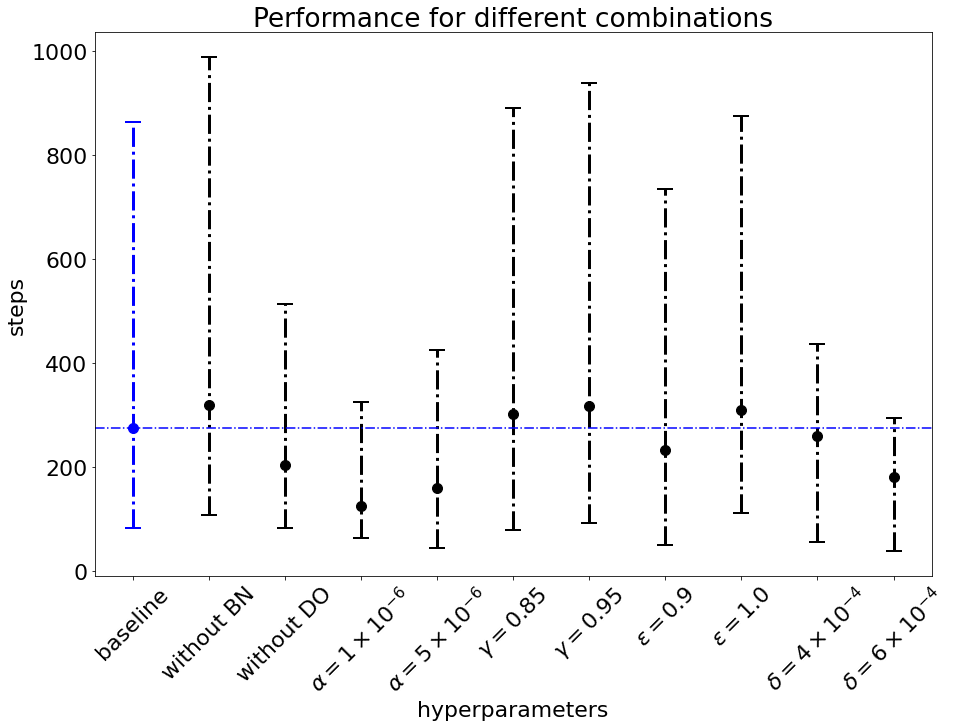
\includegraphics[width=0.9\linewidth]{figures/HP1}
    \caption{hyperparameters performance comparison}
    \label{fig:hp1}
  \end{figure}

  On top of that, since the previous work didn't apply any optimization on the training algorithm in Figure \ref{fig:code2}, they are using the default value for the batch size and memory size, i.e., $BS=1, MS=\text{length of game}$. Therefore, for these two hyperparameters, we need more exploration than the previous ones, and the performance results are shown in Figure \ref{fig:hp2}.\footnote{The tabular data can be found in \textbf{Appendix C}} 

  \begin{figure}[h!]
    \centering
    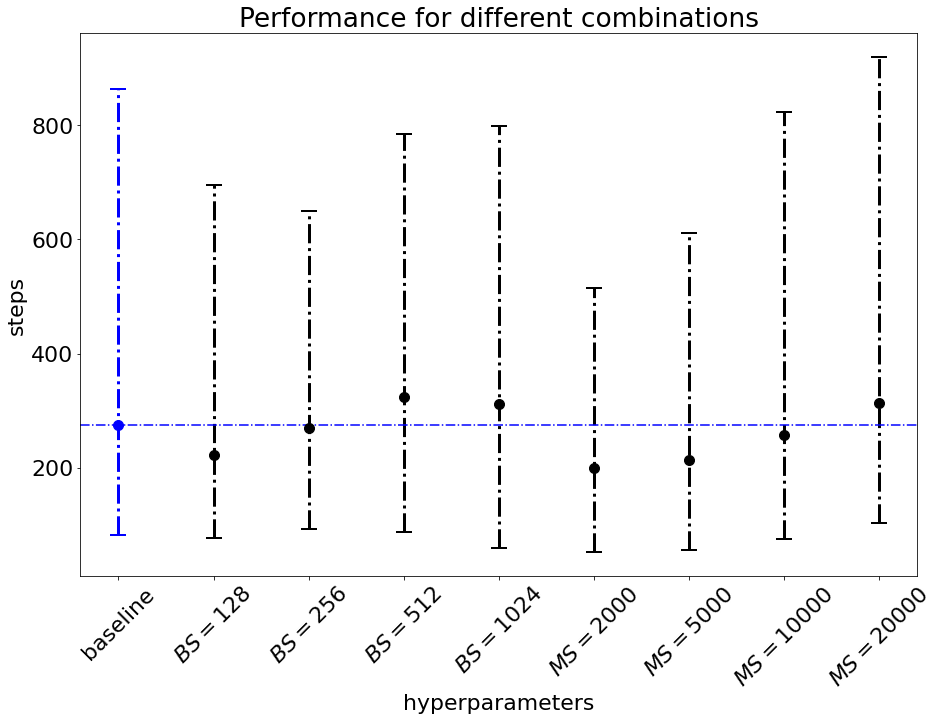
\includegraphics[width=0.9\linewidth]{figures/HP2}
    \caption{hyperparameters performance comparison}
    \label{fig:hp2}
  \end{figure}

  Comparing each combination's performance with the baseline, we expect the following hyperparameters to be an optimal combination.
  \begin{align*}
    &BN=\text{false}, DO=\text{true}, \alpha=2\times 10^{-6}, \gamma = 0.95\\
    &\epsilon=1.0,\delta=5\times 10^{-4}, BS=512, MS=20,000
  \end{align*}

  Notice that the most significant improvement comes from the removal of the batch normalization layer (which results in a $14\%$ increase in average steps) and a large memory size (which results in a $12\%$ increase in average steps). From the authors' perspective, the intuitions behind these trends are as follows:
  \begin{itemize}
    \item 
    Firstly, since we are using a combination of ReLU and leaky ReLU as activation functions for the whole network, we don't necessarily need normalization since concentration on zero doesn't help much on ReLU. Therefore, removing batch normalization will help in reducing the complexity and achieving better results.
    \item 
    On top of that, using a large memory size will help us remember more $(state, Q-value)$ pairs, which is equivalent to a larger dataset. As a result, this should also help in improving performance.
  \end{itemize}
  Now, with these hyperparameters, we indeed achieved a better validation result, as shown in Table \ref{tab:resultsSummary}, and the training curve in Figure \ref{fig:tc} also gives us some sense of why the combinations make sense. For example, a large randomization rate will dominate the early training period, so we have almost no improvement in the first half. But this is beneficial for the long term as we are exploring more and the latter half is improving a lot.
 
  \begin{figure}[h!]
    \centering
    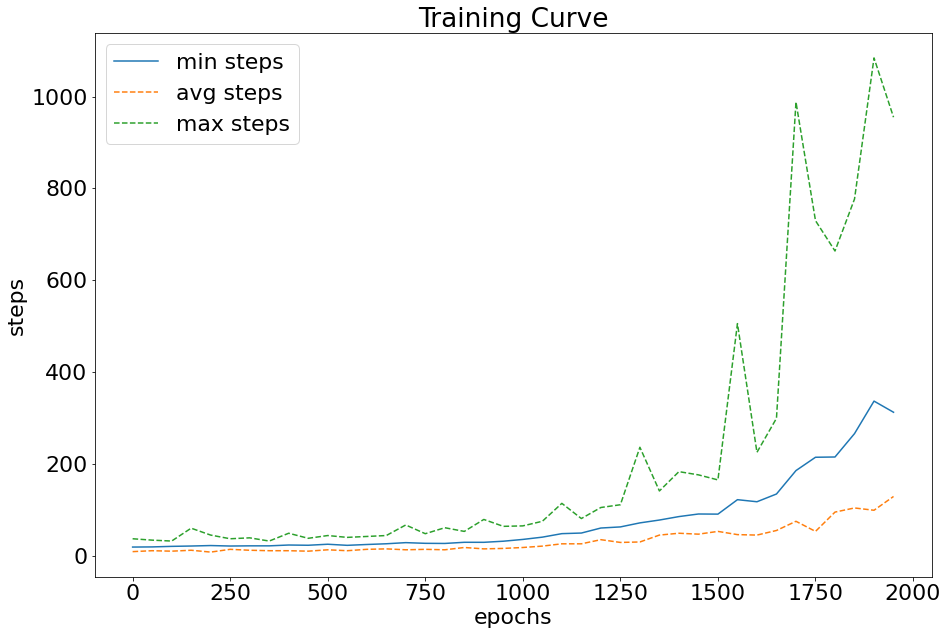
\includegraphics[width=0.9\linewidth]{figures/train_curve}
    \caption{training curve for RL agent}
    \label{fig:tc}
  \end{figure}

  Finally, with a well-trained RL agent, we could have a deeper understanding of how deep Q-learning (DQN) works by associating visual states with its q-values. A few examples can be found in \textbf{Appendix D}.
\end{itemize}

\subsection{Reflection}

As we can see in the two subsections above, our implementation is quite comprehensive in the sense that it involves numerous object-oriented programming techniques as well as some of the cutting-edge machine learning methods. Consequently, the authors will note some lessons learned during the implementation processes, and again, it naturally falls into three parts.

\begin{itemize}
  
  \item \textbf{Tetris Interface}
  
  \blue{TODO by Mongo}
  
  \item \textbf{Local Search Agent}
  
  \blue{TODO by Harry}
  
  \item \textbf{Reinforcement Learning Agent}
  
  In the authors' opinions, the most valuable lessons learned from the analysis and implementation process are that theory doesn't always correspond to the practice. In this report, we analyze how and why the reinforcement learning agent should surpass the local search agent, but after we implement both, it is later that overshadows the former. The underlying reasons will be analyzed in greater detail in the Discussion section, but in brief, the lesson is that the most complex model isn't necessarily the best model. On top of that, the authors also learned many practical skills during the learning and implementation process. Firstly, none of the authors had any preknowledge about q-learning, so we need to study everything from scratch by ourselves. This learning process should be beneficial for further career, either in academics or industry. Moreover, during the implementation process, the authors encountered plenty of challenges that will never show up in the homework — for example, spending days training and validating to find optimal hyperparameters, spending hours dealing with the frequent switch between CPU and GPU, etc. These experiences give us a more in-depth understanding of Reinforcement Learning as well as practice our problem-solving skills in real life. 
\end{itemize}
% {\bf Complete this section for D2 and D3.}

% The {\it Results} section ($\sim$2 pages) describes how you evaluated the algorithms and reports the findings.  

% {\bf Complete the following two paragraphs for D2.}



% {\bf Complete the following two paragraphs for D3.}

% Describe the findings from your evaluation.  Describe both (a) how well your techniques worked, and (b) what you learned about the problem through these techniques.  

% Prepare figures (e.g., Figure \ref{fig:results2}) and tables (e.g., Table \ref{tab:results1}) to describe your results clearly.  Make sure to label your figures and tables and explain them in the text.  If you are comparing the performance of algorithms, include statistical tests to assess whether the differences are statistically significant.  If possible, describe how your techniques compare to prior work.  

% \begin{table}[h!]
%     \centering
%     \normalsize{
%     \begin{tabular}{ l c }
%     \hline
%          Techniques & F-1 Score\\
%          \hline
%           Baseline & 0.80 \\
%           Another Baseline & 0.76\\
%           My Awesome Algorithm & {\bf 0.95}\\
%          \hline
%     \end{tabular}}
%     \caption{example of a table summarizing the results}
%     \label{tab:results1}
% \end{table} 

% \begin{figure}[htbp!]
%   \centering
%   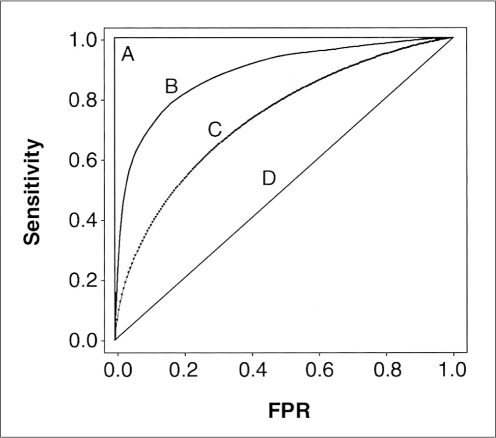
\includegraphics[width=0.9\linewidth]{figures/roc.png}
%   \caption{ROC curve of my awesome algorithms}
%   \label{fig:results2}
% \end{figure}


%%%%%%%%%. Discussion %%%%%%%%%

% \section{Discussion}

% {\bf Complete this section for D4.}

% The {\it Discussion} section ($\sim$1 pages) describes (a) the implications of your results, and (b) the impact and the limitations of your approach.  

% For the results, describe how a reader should interpret them.  Try to form concise take-away messages for the reader.  For your approach, describe the extent to which your approach helps to solve the problem.  Describe any limitations of your approach.  If possible, compare your results and your approach to that of prior work. 

%%%%%%%%%. Conclusion %%%%%%%%%

% \section{Conclusion}

% {\bf Complete this section for D4.}

% The {\it Conclusion} section ($\sim$0.5 pages) provides a brief summary of the entire paper.  In this section, describe 
% \begin{itemize}
%     \item the motivation, the problem, and your results, and
%     \item 3-4 promising future directions.
% \end{itemize}

%%%%%%%%% Bibliography %%%%%%%%%
\newpage
\bibliographystyle{aaai}
\bibliography{report}




\begin{figure*}[b!]
  \centering
  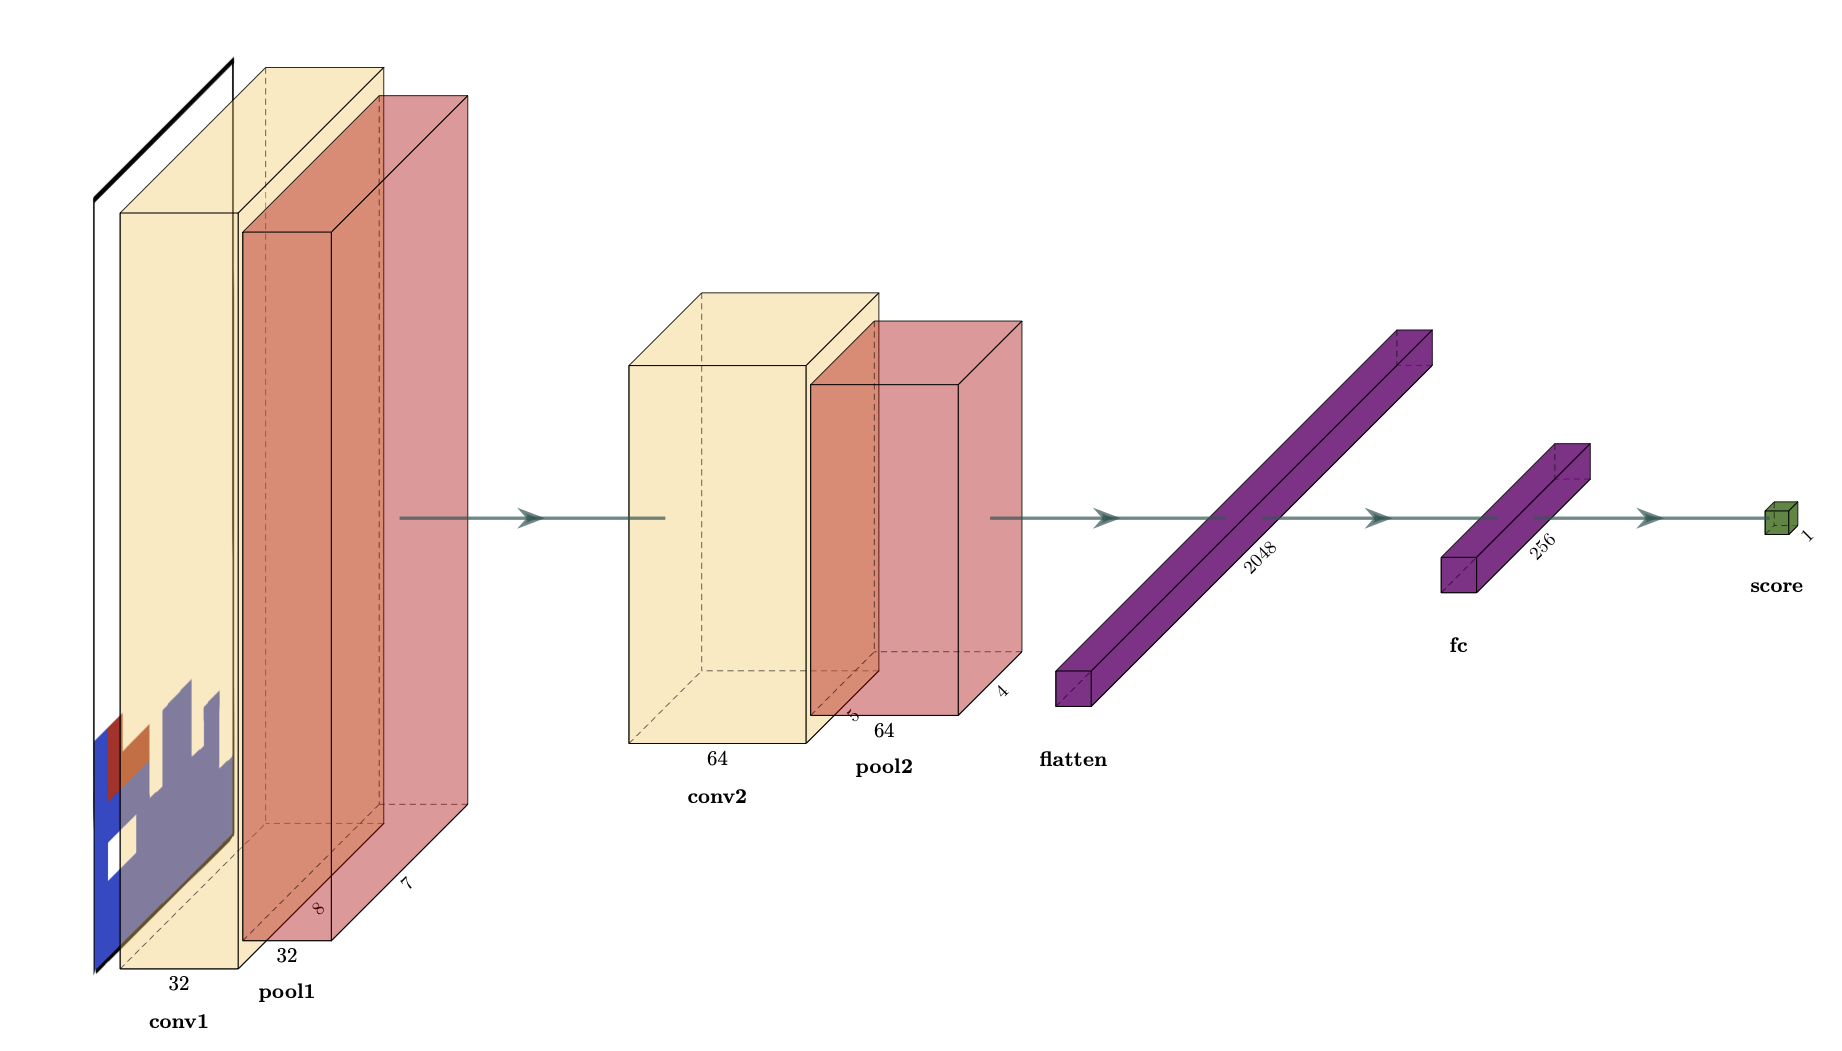
\includegraphics[width=0.75\linewidth]{figures/DQN.png}
  \caption{Deep Q-network architecture}
  \label{fig:DQN}
\end{figure*}
\newpage
$\,$
\newpage
\section{Appendix A}

The structure of the network is shown in the Figure \ref{fig:DQN} and here are the detailed information about each layer:

\begin{itemize}
  \item 
  {\bf conv1}: a convolutional layer with filter size $3\times 3$, output channel size $32$, and leaky ReLU activation function.
  \item 
  {\bf pool1}: a max-pooling layer with filter size $2\times 2$.
  \item 
  {\bf conv2}: an identical layer as {\bf conv1} except that the output channel size to be $64$.
  \item 
  {\bf pool2}: an identical layer as {\bf pool2}.  
  \item 
  {\bf flatten:} this is simply a flattened version of the {\bf pool2} feature map.
  \item 
  {\bf fc}: this is a fully connected layer of size $256$ with ReLU activation function.
  \item 
  {\bf score}: this is a fully connected layer of size $1$ with ReLU activation function.
\end{itemize}

\newpage
\section{Appendix B}

  The sequential training process of \textit{training by part} is actually not as easy as it sounds like, and the main problem here is the difference in length of the flattened vectors:

  \begin{table}[h!]
    \centering
    \normalsize{
      \begin{tabular}{ |c|c| } 
        \hline
        Input Size & Flattened Vector Size  \\ 
        \hline
          $5\times 10$ & $512$  \\ 
          \hline
          $10\times 10$ & $1024$  \\ 
          \hline
          $20\times 10$ & $2048$  \\
          \hline
        \end{tabular}}
    \caption{Flattened vector sizes for different input}
    \label{tab:vectorSize}
  \end{table} 

  The difference between these vectors' sizes will mess up the weight matrix of DQN architecture, so we need to initialize the weight matrix manually when we change the input size. More precisely, whenever we increase the input size, we will initialize a new fully-connected layer and copy the previous network's weights to half of the current network. A visualization for $5\times 10$ to $10\times 10$ is shown in Figure \ref{fig:training}, where we initialize the bottom half (shown in blue) of the weight matrix with the previous weights and randomly initialize the upper half of the weight matrix (shown in green).

  \begin{figure}[h!]
    \centering
    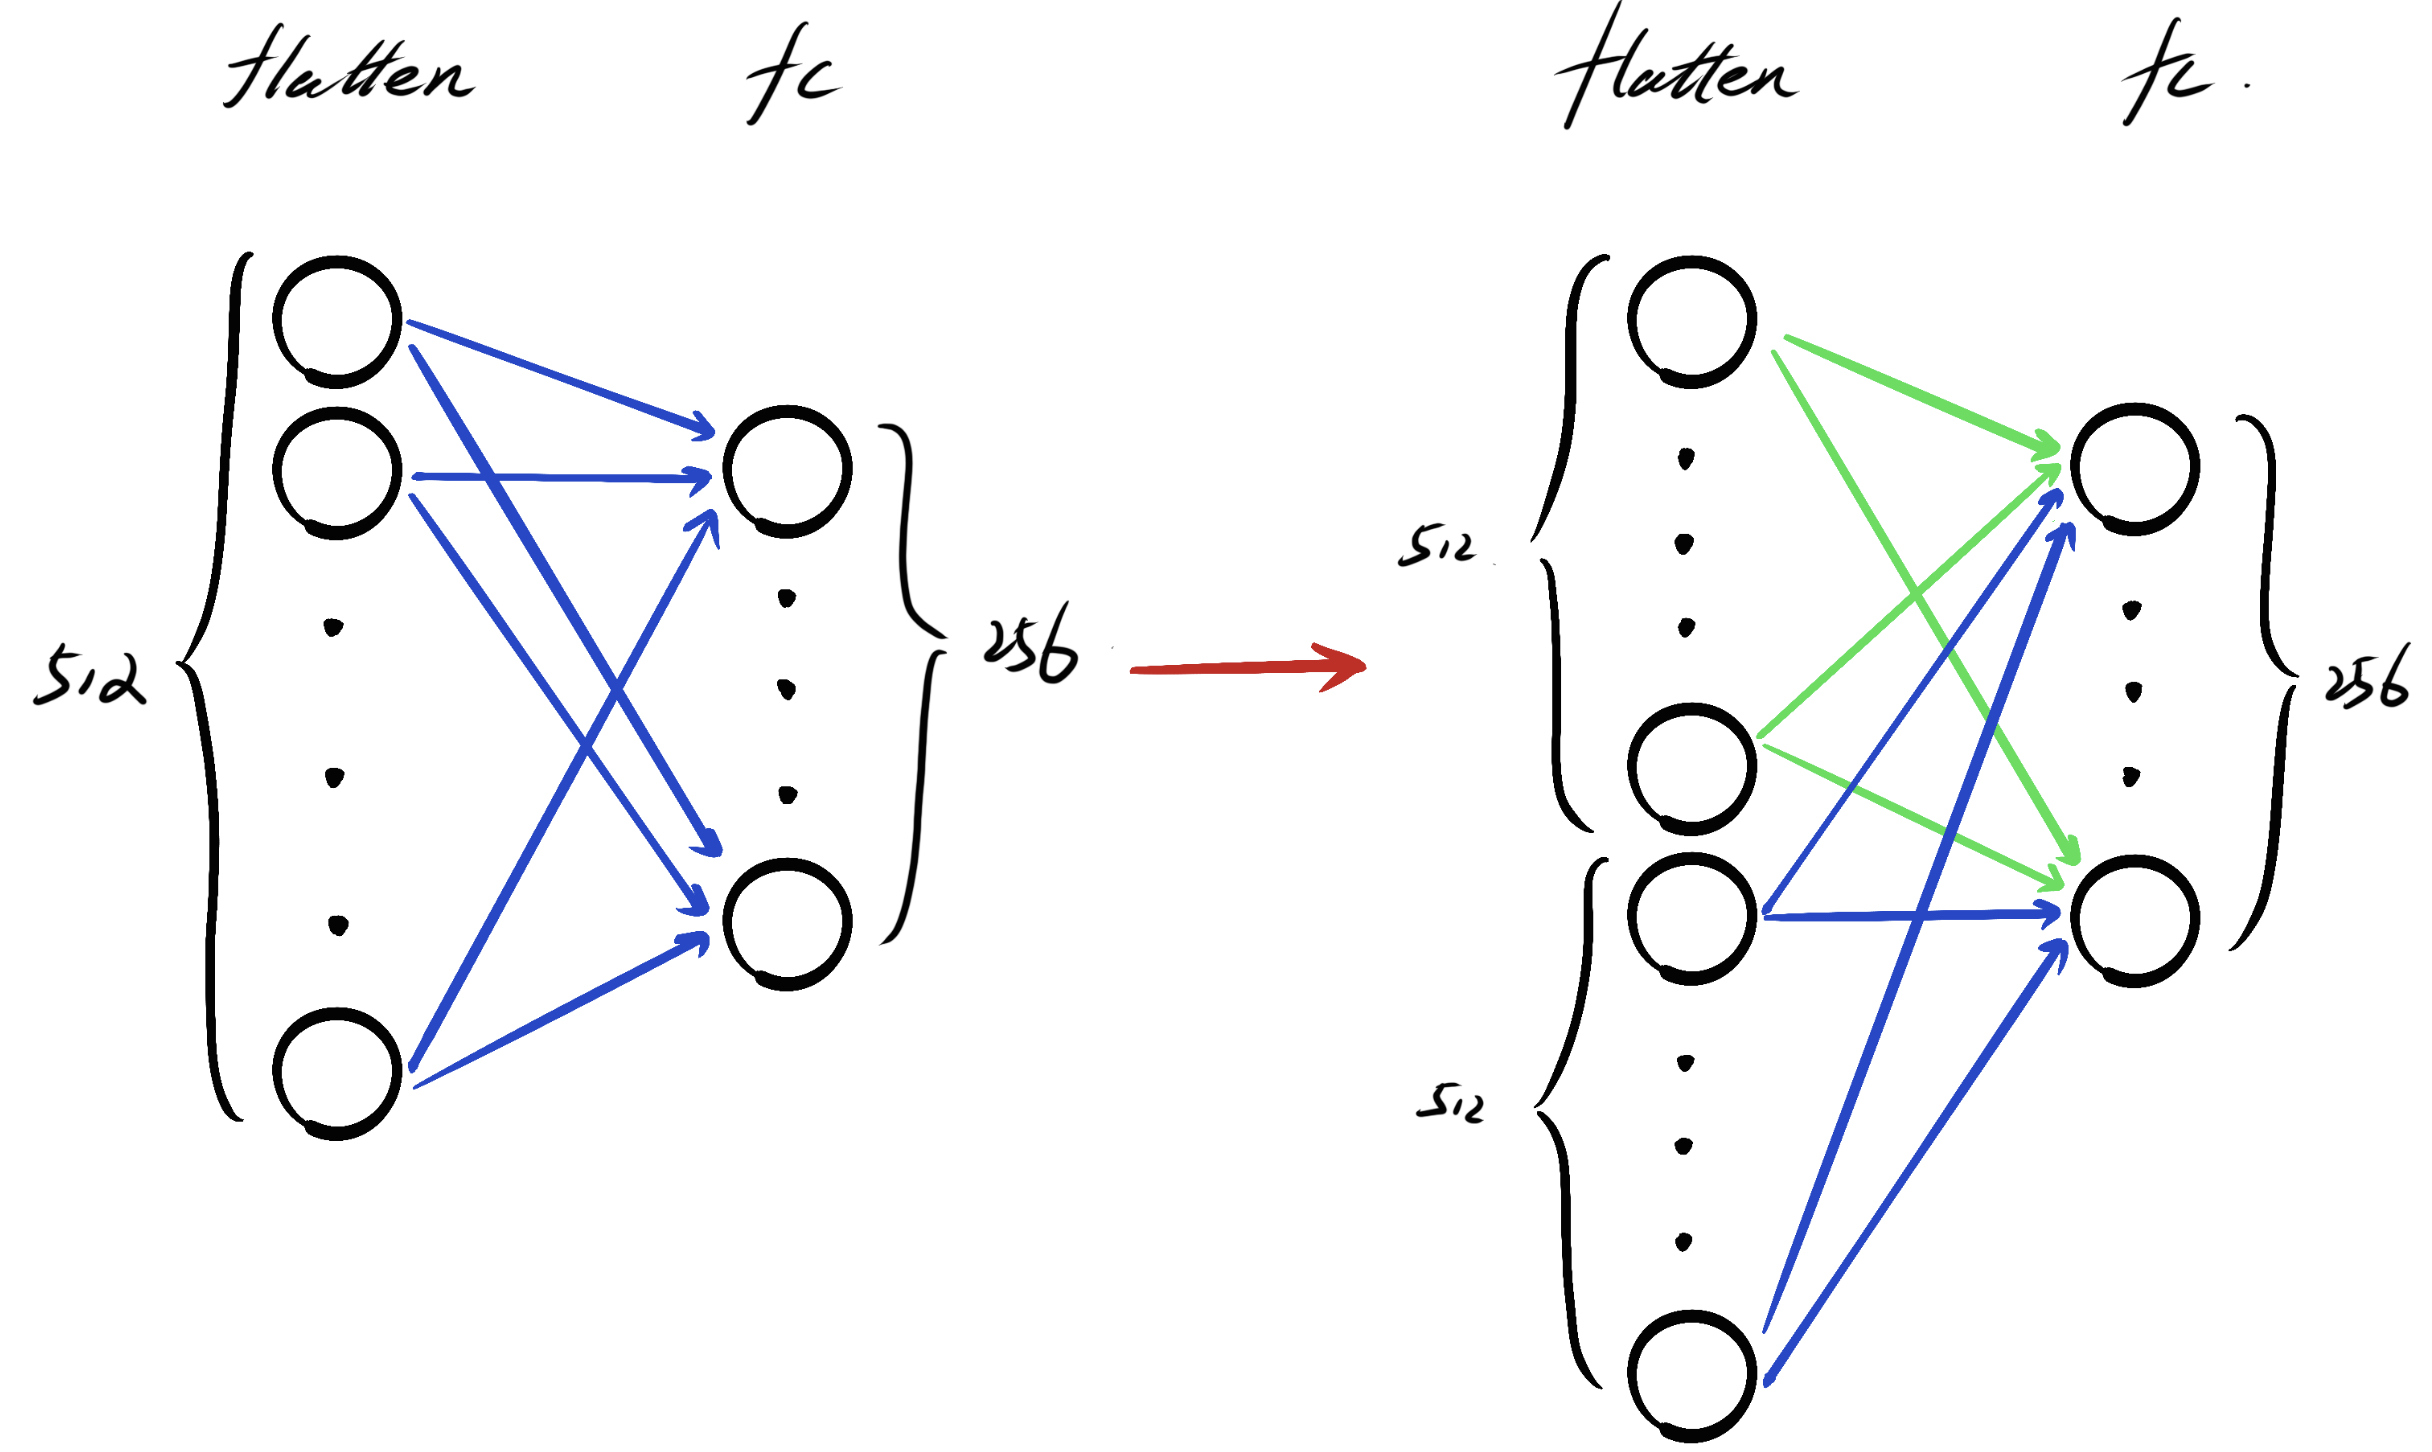
\includegraphics[width=0.75\linewidth]{figures/architecutre.jpeg}
    \caption{Grouped action example}
    \label{fig:training}
  \end{figure}
  
  \newpage
  \section{Appendix C}
  \begin{table}[h!]
    \centering
    \normalsize{
      \begin{spacing}{1.9}
      \begin{tabular}{ |cccc| } 
        \hline
        features & min steps & avg steps & max steps  \\ 
        \hline
        \hline
        baseline & $83$& $274.39$ & $863$\\
        without $BN$&$108$&$319.15$&$988$\\
        without $DO$&$82$&$203.91$&$513$\\
        $\alpha=1\times 10^{-6}$&$63$&$124.26$&$325$\\
        $\alpha=5\times 10^{-6}$&$45$&$158.41$&$425$\\
        $\gamma=0.85$&$78$&$300.02$&$890$\\
        $\gamma=0.95$&$92$&$318.87$&$938$\\
        $\epsilon=0.9$&$50$&$232.81$&$734$\\
        $\epsilon=1.0$&$112$&$310.59$&$874$\\
        $\delta= 4\times 10^{-4}$&$56$&$258.59$&$437$\\
        $\delta= 6\times 10^{-4}$&$38$&$180.19$&$295$\\
        $BS=128$&$77$&$224.45$&$695$\\
        $BS=256$&$93$&$267.91$&$650$\\
        $BS=512$&$88$&$325.05$&$785$\\
        $BS=1024$&$59$&$311.92$&$798$\\
        $MS=2000$&$53$&$196.30$&$515$\\
        $MS=5000$&$55$&$212.99$&$612$\\
        $MS=10000$&$75$&$257.16$&$823$\\
        $MS=20000$&$103$&$312.34$&$919$\\
        \hline
      \end{tabular}
    \end{spacing}
    }
    \caption{Tabular Results for RL Agent}
    \label{tab:tabularResult}
  \end{table}  
  \newpage
  \section{Appendix D}

  \begin{figure}[h!]
    \centering
    \subfigure[score=1.94128]{
    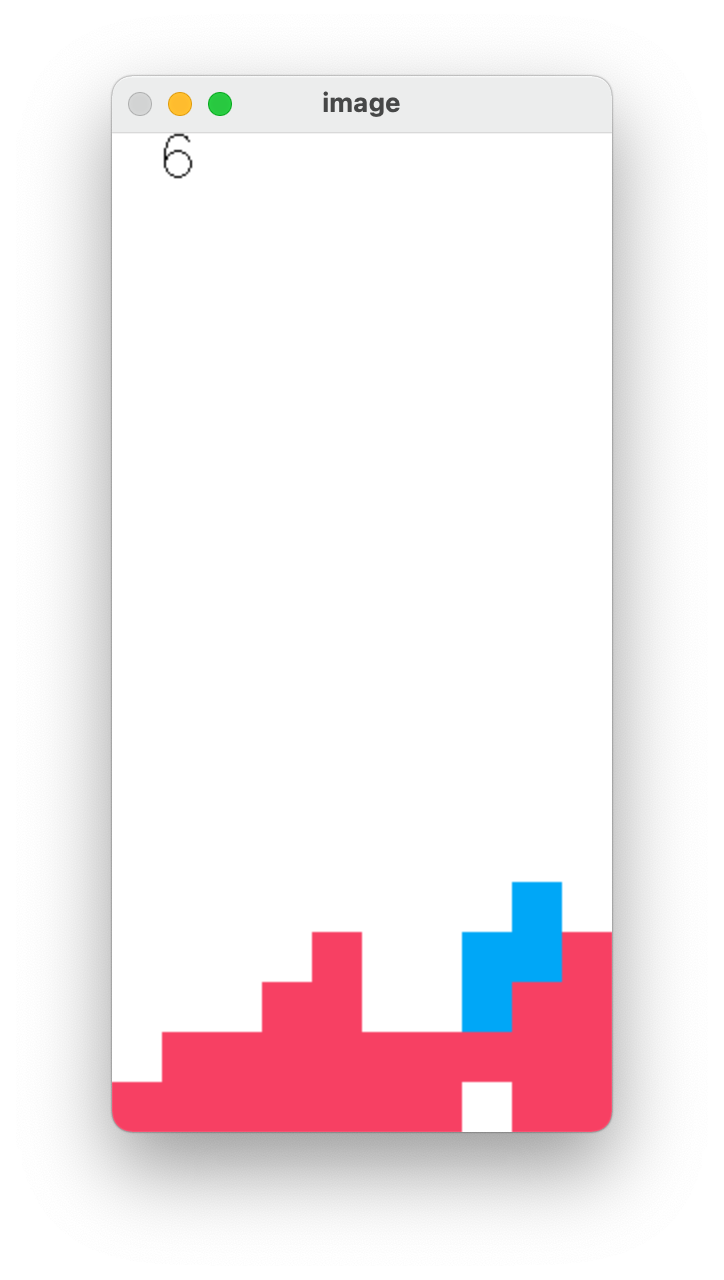
\includegraphics[width=0.19\textwidth]{figures/example1.png}
    }\hfill
    \subfigure[score=2.34137]{
    
\includegraphics[width=0.19\textwidth]{figures/example2.png}
    }
    \subfigure[score=1.13586]{
    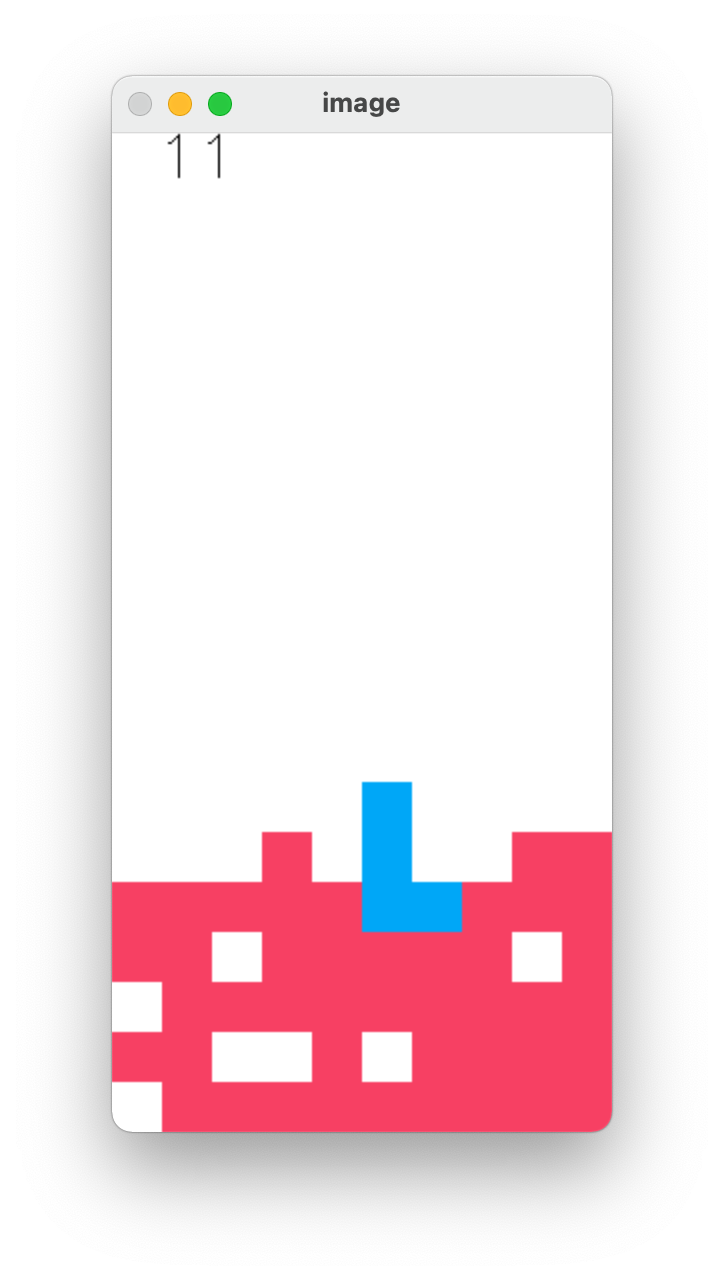
\includegraphics[width=0.19\textwidth]{figures/example3.png}
    }\hfill
    \subfigure[score=0.96125]{
    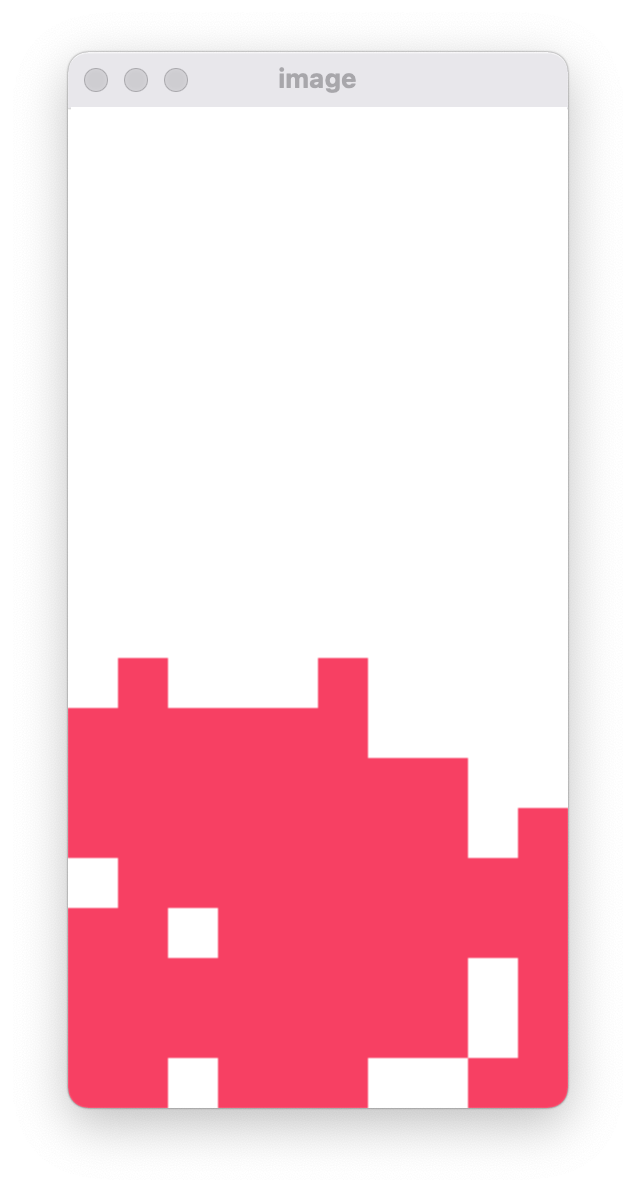
\includegraphics[width=0.19\textwidth]{figures/example4.png}
    }
    \subfigure[score=-0.80523]{
    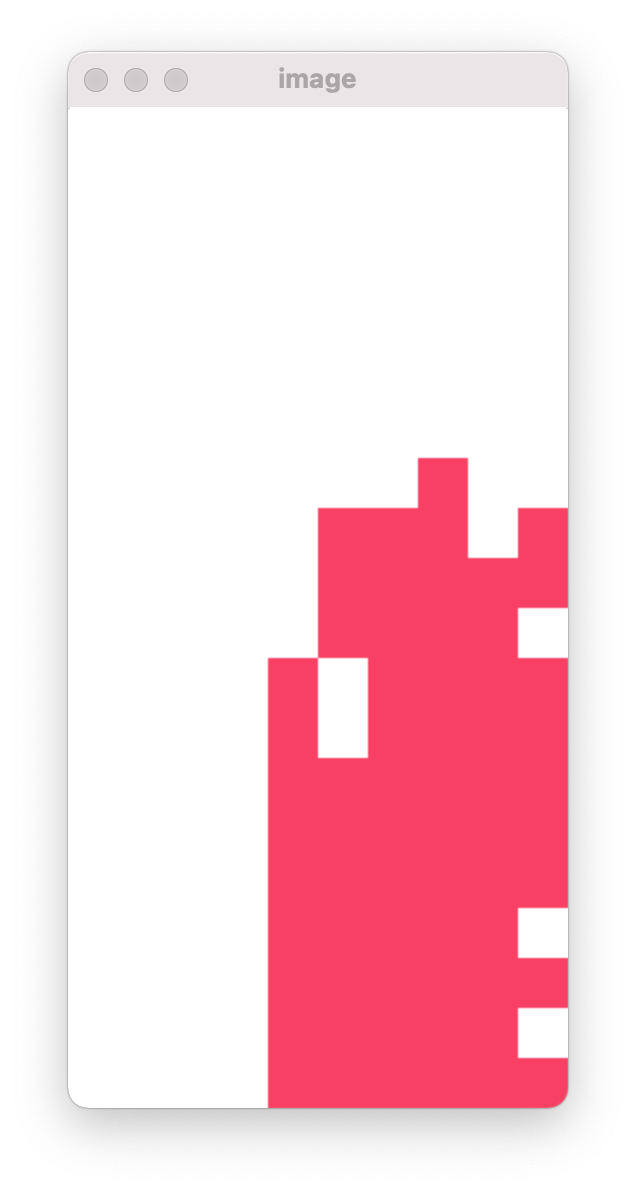
\includegraphics[width=0.19\textwidth]{figures/example5.png}
    }\hfill
    \subfigure[score=-0.79563]{
    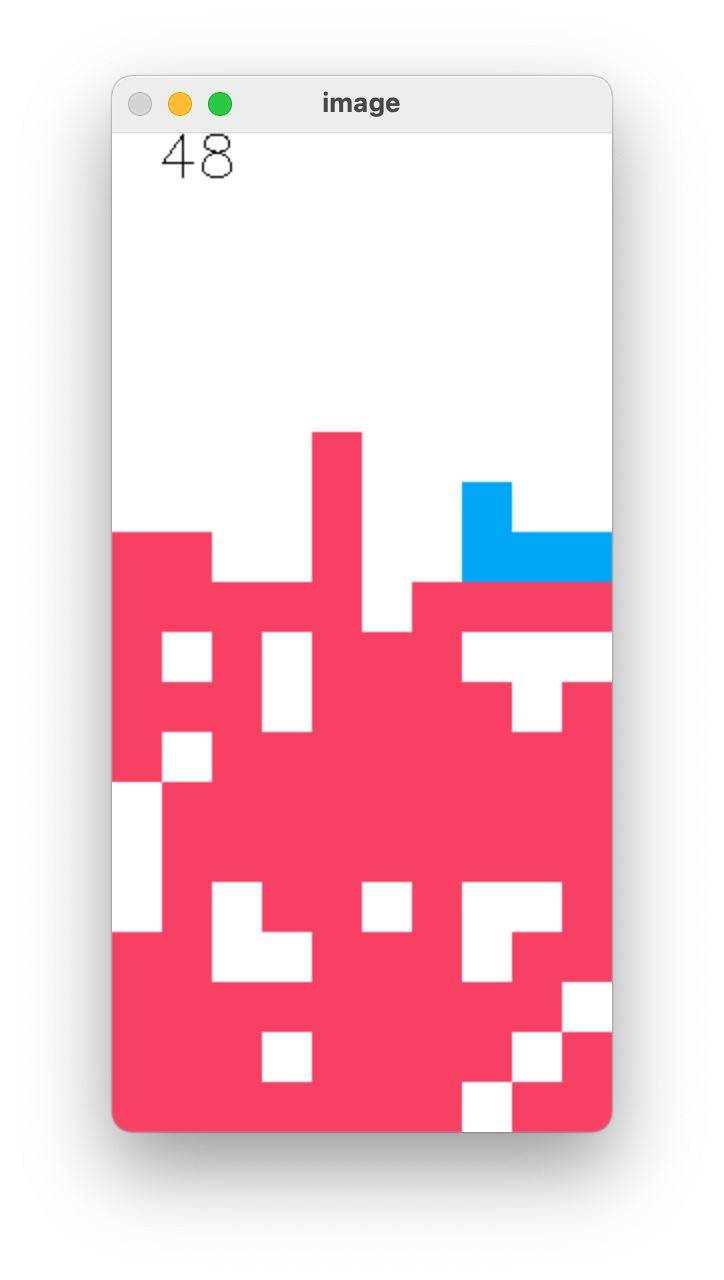
\includegraphics[width=0.19\textwidth]{figures/example6.png}
    }
    \caption{Scores for some sample states}
  \end{figure}
\end{document}
